\chapter{Studies of Displaced Jet Tagging Variables}

\section{Introduction}


The identification of jets originating from $b$ quarks ($b$-tagging) was originally developed and successfully utilized for the discovery of the top quark.
 Among other applications, $b$-tagging is now a tool for studying the Higgs and searching for beyond the standard model (BSM) physics.
 Since its inception, $b$-tagging has evolved including the implementation of particle flow, refined secondary vertex algorithms, and advanced multivariate techniques. 
The strength of $b$-tagging is not restricted to its signal to background differentiation, but includes the community sized impact of a well defined and supported physics o
bject definition. 

The $b$-tagging algorithms are publicly documented with corresponding working points and data/mc factors derived by the physics object group (POG in CMS). 
The algorithms are integrated directly into the experiment software allowing fast adoption of subsequent improvements.  The object can then be
used interchangeably as part of a large toolkit of jets, leptons, taus, photons, and missing energy. 

Past searches (list references here) by CMS and ATLAS experiment for long lived particles decaying to jets rely significantly 
on secondary vertexing of displaced tracks. As the ability to vertex the jet is highly dependent on the ability to reconstruct 
highly displaced tracks, the existence of a vertex, although the  highly separating between signal and background is often the most inefficient selection criteria
 (especially at long life times on the scale of the detector). Of particular concern is that current vertexing algorithms may not 
 perform effectively for non-SM jet vertices such as found in Emerging Jets [citation].

The case of long lived particle that decay outside of the detector remains outside the scope of jet-tagging, but remains an interesting use 
case in conjunction with the tag definitions. 

Analyses utilizing the tags should expect strong topological sensitivity for $\geq 2$ displaced jets, electrons, and taus regardless of their
configuration of a long lived $X$ decay. Lifetime sensitivity is expected for decays which occur for transverse distances between ~$1$mm to ~$2$m,
corresponding to outside of the lifetime of b hadrons up to the edge of the HCAL.


\subsection{Significant differences with respect to b-tagging}

Given the close analogy to $b$-tagging techinques, it is important to clarify where $b$-tagging algorithms are inefficient and where they can be exteded.

For shorter lifetime regimes ($c\tau < 1$ mm), $b$-tagging  can still identify displaced jets, but leaves room for new techniques. 
Heavy long-lived resonsances undergoing a 2 body decay will have significantly more momentum transverse to the flight direction of the long lived particle (when compared to a $b$ decay). This angle is a powerful discriminant to background nuclear interactions and is strongly correlated with the boost of the mother particle. 
Under the assumption that the angle is small, $b$-tagging uses only positively signed impact parameters for track identification (corresponding to to decays downstream of the flight path). Heavy particles produced 
nearly at rest will decay isotropically with impact parameters of negative sign (when decays occur backward relative to the mother's momentum direction). 

For longer lifetimes, a transition occurs at distances larger than a few centimeters where new issues undaddressed by b-tagging arise. Although the $b$ meson is displaced
it is comparably straightforward to decern the primary vertex of the event. This allows b-tagging algorithms to more accurately calculate longitudinal quantities, such as 3D track impact parameters. 
For displaced jets, this is not the case  and utilizing longitudinal quantities 
relative to a mis-identified primary vertex can yield sub-optimal performance. 
Pixel hit requirements are explcitly required for tracks used in $b$-tag secondary vertexing,
 but displaced jets decays can occur outside the pixel layers. In addition, b-tagging algorithms include upper bounds on
 longitudinal and transverse impact parameters to limit contributions from nuclear interactions. 


o
\section{Samples}

\section{Signal Samples}

\begin{figure}
\begin{center}
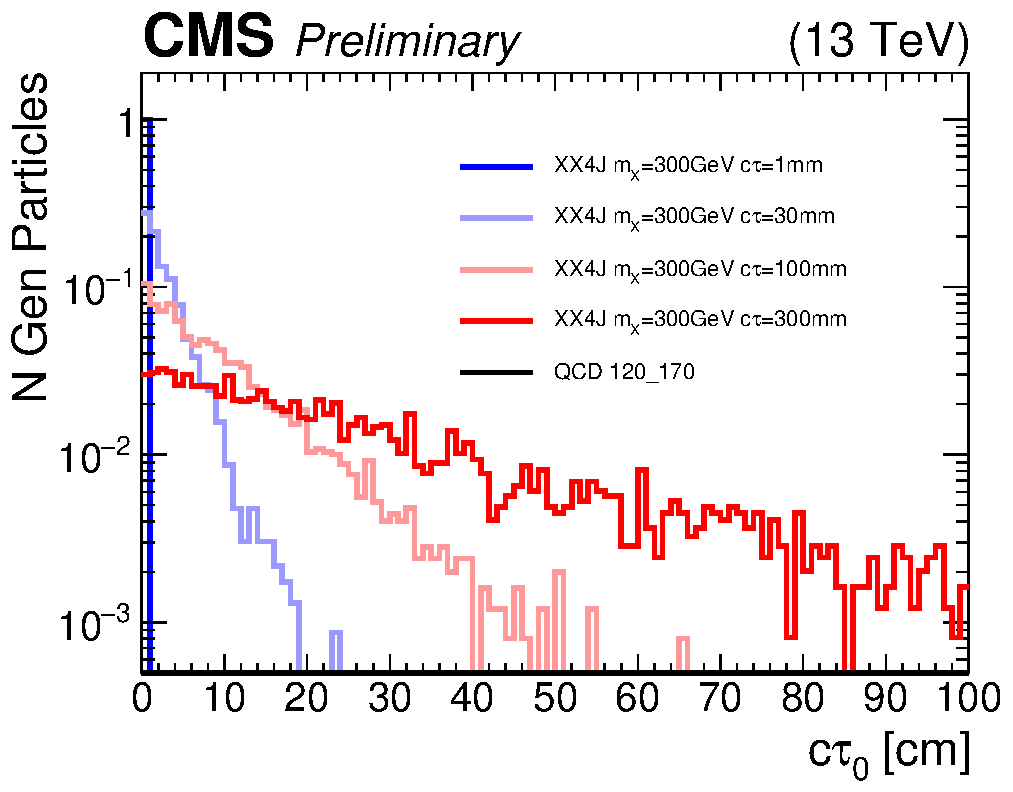
\includegraphics[width=.45\textwidth]{figures/an_jetid/VTX_MATCH_IP/XX4J_ctau0}
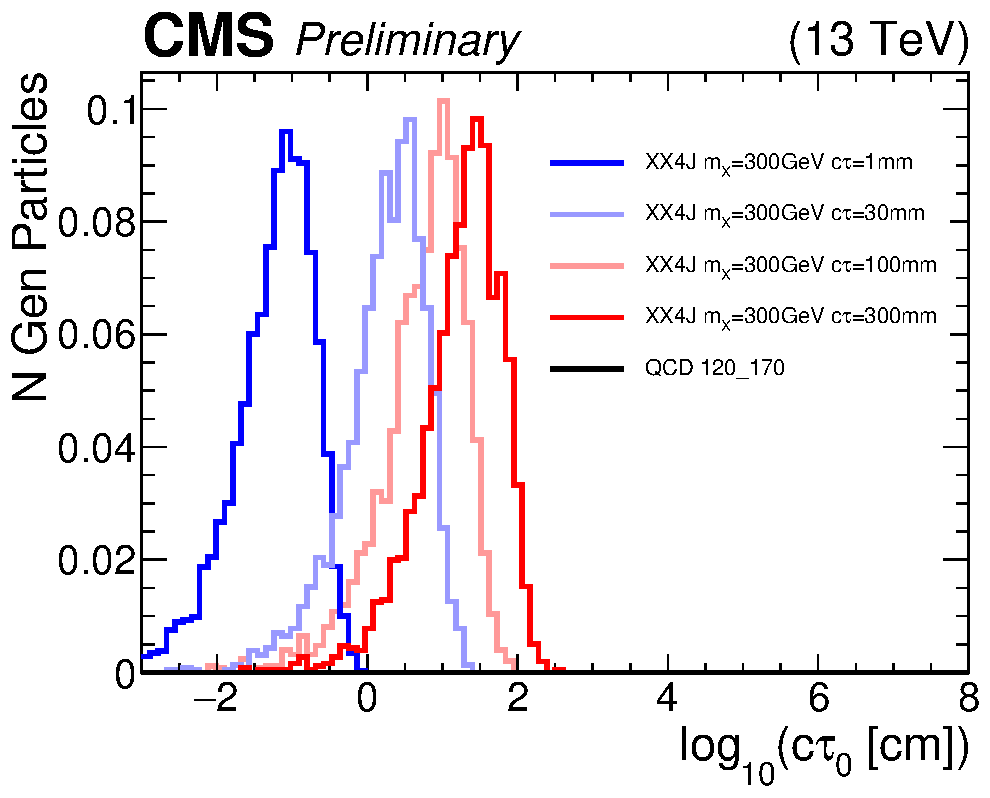
\includegraphics[width=.45\textwidth]{figures/an_jetid/VTX_MATCH_IP/XX4J_log_ctau0}
\end{center}
\caption{The proper $c\tau_0$ of the XX4J samples. The samples are generated with exponential lifetime distributions
$e^{- x / c\tau_0}$ which have mean $c\tau_0$ and exponential slope $1/c\tau_0$.}
\label{fig:xx4j_ctau0}
\end{figure}

Two signal samples are used to study displaced identification which we will refer to as $XX4J$ and $GUN$. Both samples are generated
using PYTHIA 8 (cite-pythia). 

\begin{figure}
\begin{center}
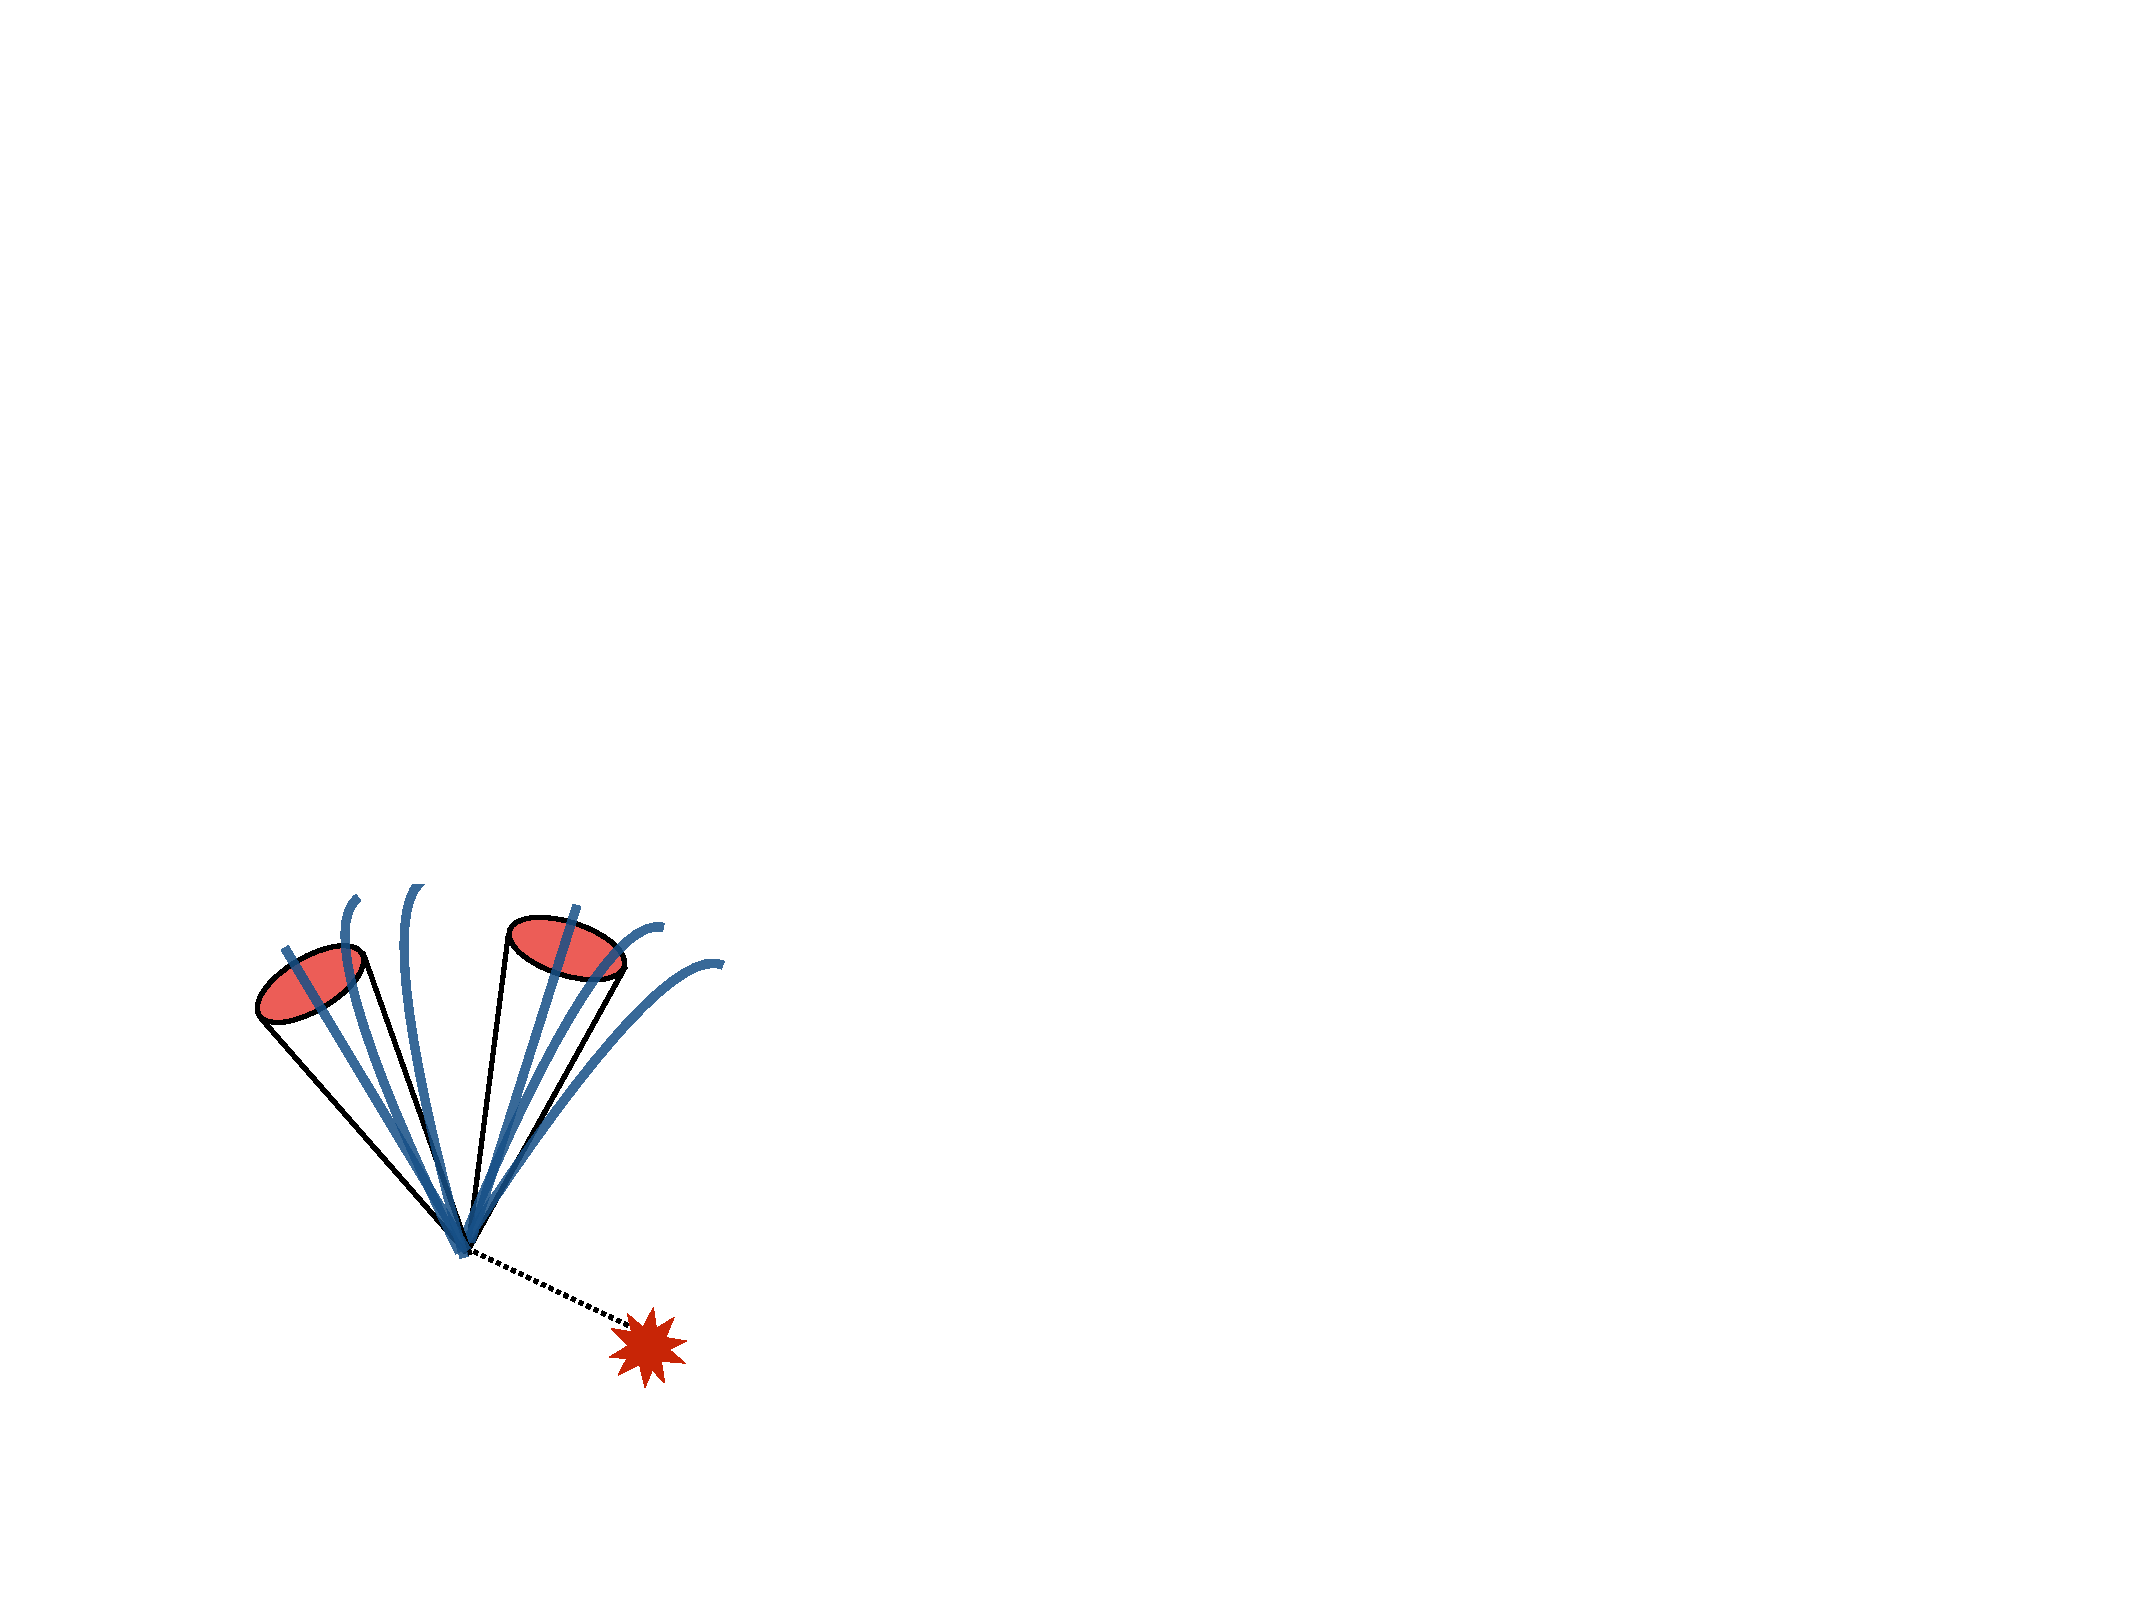
\includegraphics[width=.38\textwidth]{figures/an_jetid/DIAGRAMS/dijet_gun}
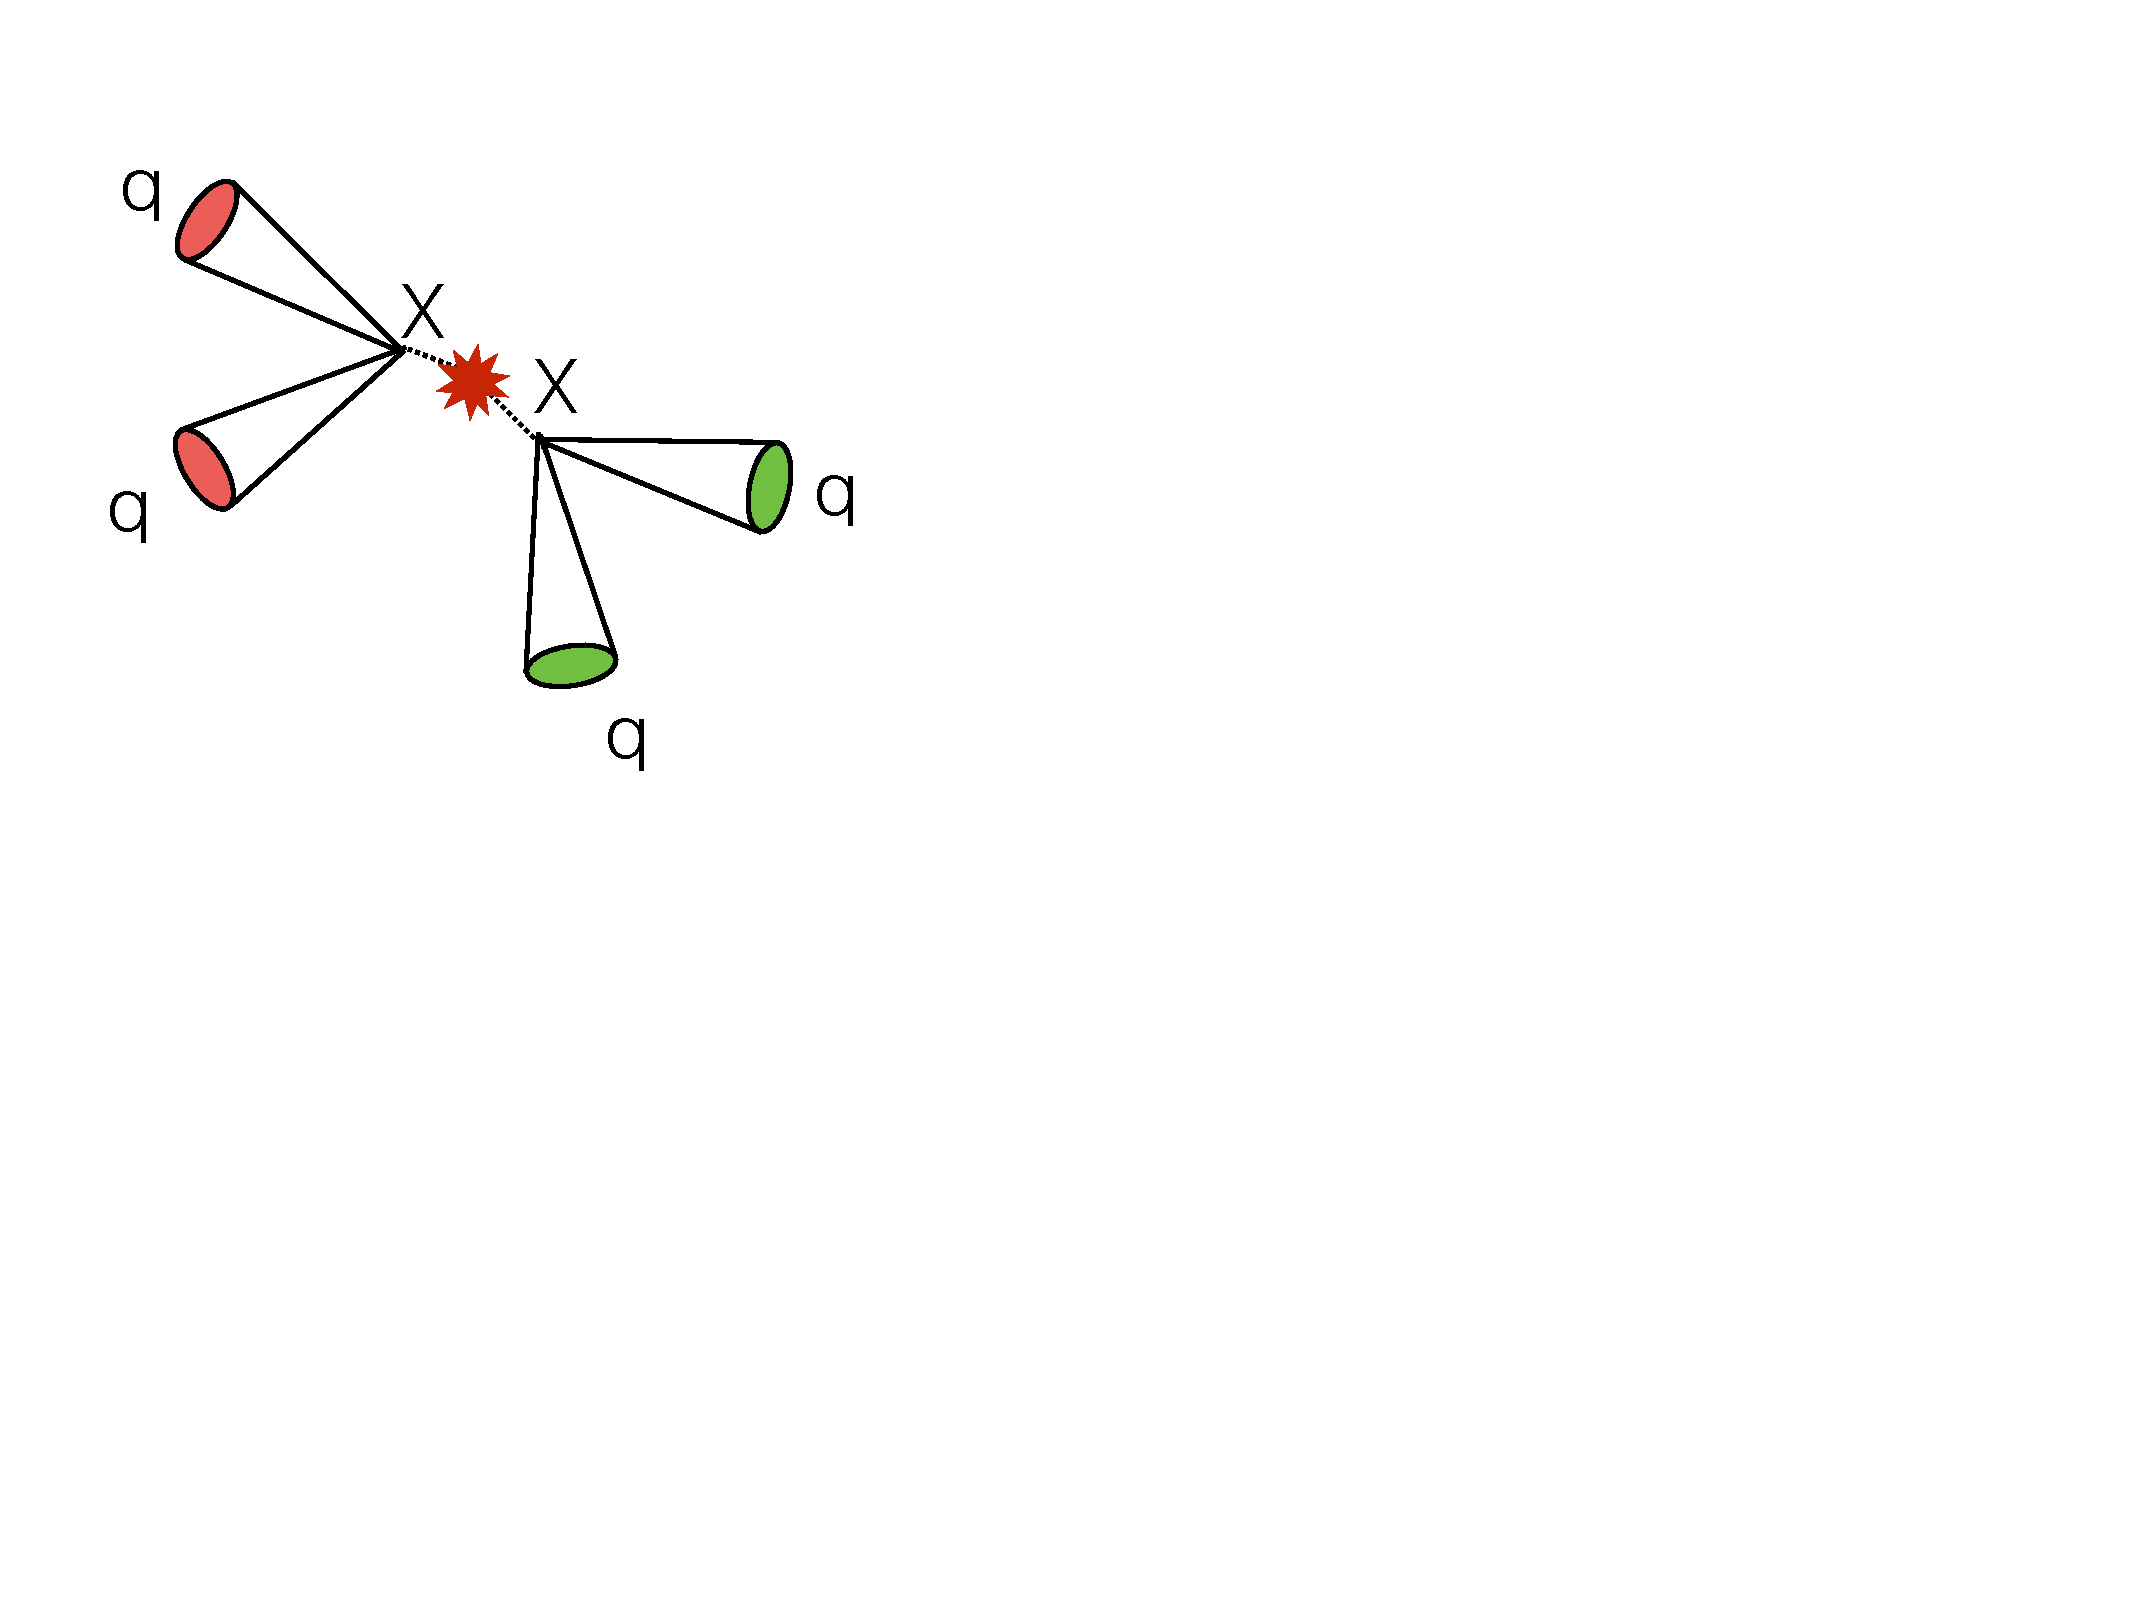
\includegraphics[width=.58\textwidth]{figures/an_jetid/DIAGRAMS/xx4j_diagram}
\end{center}
\caption{The topology of the two samples used in the study $GUN$ (left) and  $XX4J$ (right) }
\label{fig:xx4j_gun}
\end{figure}

The $XX4J$ sample consists of the direct pair production of two neutral $X^{0}$'s with finite lifetime.  
Each $X^{0}$ decays to u,d,s,c, and b with equal probability. This
sample is generated with flat pileup between 10 and 50 with 25 ns bunch crossing code for cmsDriver as
  \texttt{Flat\_10\_50\_25ns}. It is important
to note that due to pile up interactions, these samples contain both prompt and displaced jets. 
In this sample, variables for displaced jet identification generally have two distinct populations of jets. 

The $XX4J$ samples are generated with varied lifetimes and masses (Fig. \ref{fig:xx4j_ctau0}). Each $X^0$ has an
 exponential lifetime distribution $e^{-x / c\tau_0}$ with mean $c\tau_0$ and slope $1/c\tau_0$. 

The second sample is a displaced di-jet gun sample denoted $GUN$. This sample is generated using the \texttt{PythiaPtGun} interface. A single $X^0$ 
particle is generated with flat $50 < p_{t} < 500$~GeV, flat $\phi$, and flat $-2.4< \eta < 2.4$. The $X^{0}$ decays to a pair of 
d quarks with 100\% branching fraction. Each event will thus contain a single displaced vertex. 
The configuration for the gun parameters is shown below. Small modifications to CMSSW are required to create a Pythia rather than HEPMC Particle
with a finite lifetime. 

%% \begin{verbatim}
%%     PGunParameters = cms.PSet(
%%         ParticleID = cms.vint32(35),
%%         AddAntiParticle = cms.bool(False),
%%         MinPhi = cms.double(-3.14159265359),
%%         MaxPhi = cms.double(3.14159265359),
%%         MinPt = cms.double(50.0),
%%         MaxPt = cms.double(500.0),
%%         MinEta = cms.double(-2.4),
%%         MaxEta = cms.double(2.4)
%%         ),}
%% \end{verbatim}

The resonance is decayed within pythia and passed directly to hadronization bypassing all process level pythia effects: initial
state radiation, final state radation, and beam remnants. Furthermore, the event is reconstructed without pileup mixing. This sample
is generated to have a sample of reconstructed tracks that only originate from a displaced vertex without the complications
of correctly. One important side effect of simulating without pileup is the lack of a reconstructed primary vertex. 

\begin{figure}
\begin{center}
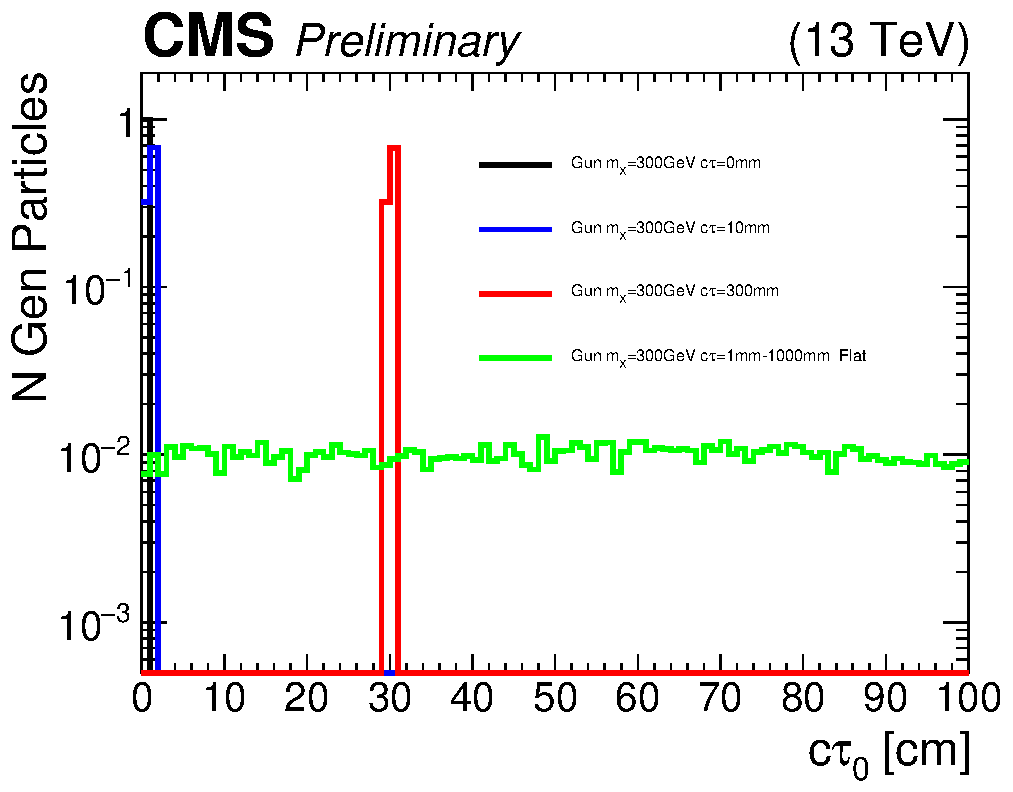
\includegraphics[width=.45 \textwidth]{figures/an_jetid/VTX_MATCH_IP/GUN_ctau0}
\end{center}
\caption{The proper $c\tau_0$ of the displaced di-jet gun samples. The samples are generated with either flat, or delta function
$\delta(c\tau_0 - c\tau_0')$ lifetime distributions}
\label{fig:gun_ctau0}
\end{figure}

The proper lifetime distribution of the sample is chosen to be either a delta function $\delta(c\tau_0 - c\tau_0')$ or 
flat between 1mm and 1000mm (Fig. \ref{fig:gun_ctau0}). Additionally two prompt dijet gun samples are built for comparison.
One sample with lifetime 0mm decaying to two b-quarks and one sample with lifetime 0mm decaying to two d-quarks. A reminder
that the decay length in the lab frame will differ by a factor $\gamma\beta$ from the proper lifetime . 

%% \begin{figure}
%% \begin{center}
%% 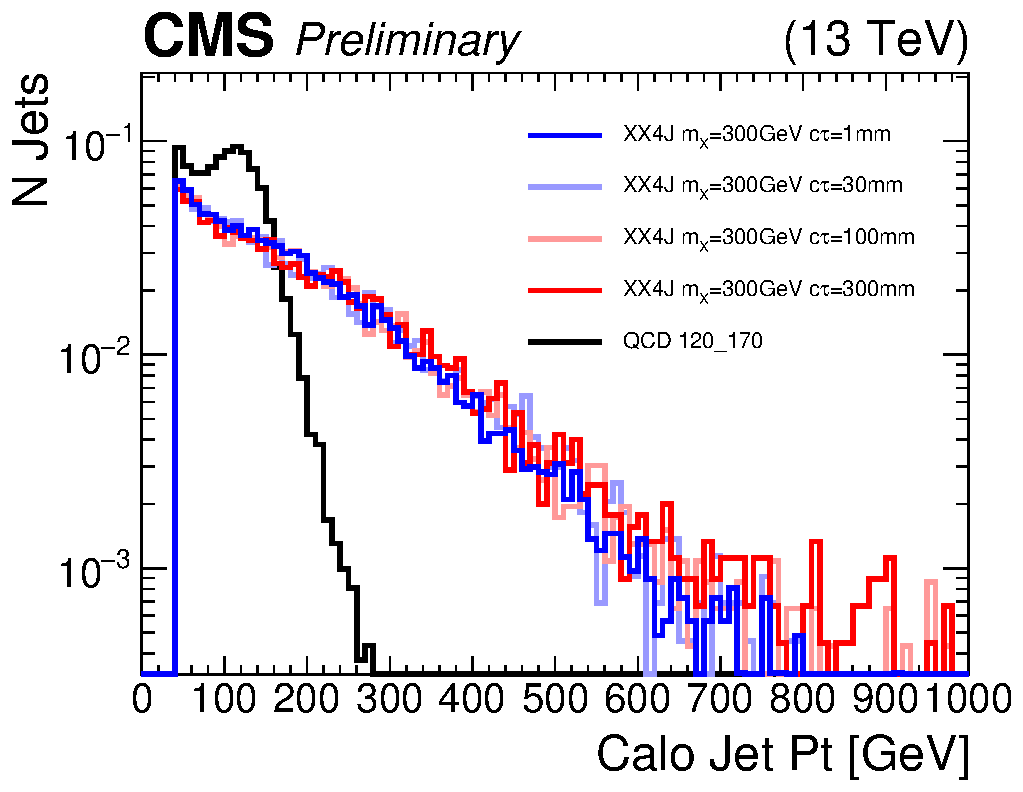
\includegraphics[width=.45\textwidth]{figures/an_jetid/VTX_MATCH_IP/XX4J_caloJetPt}
%% 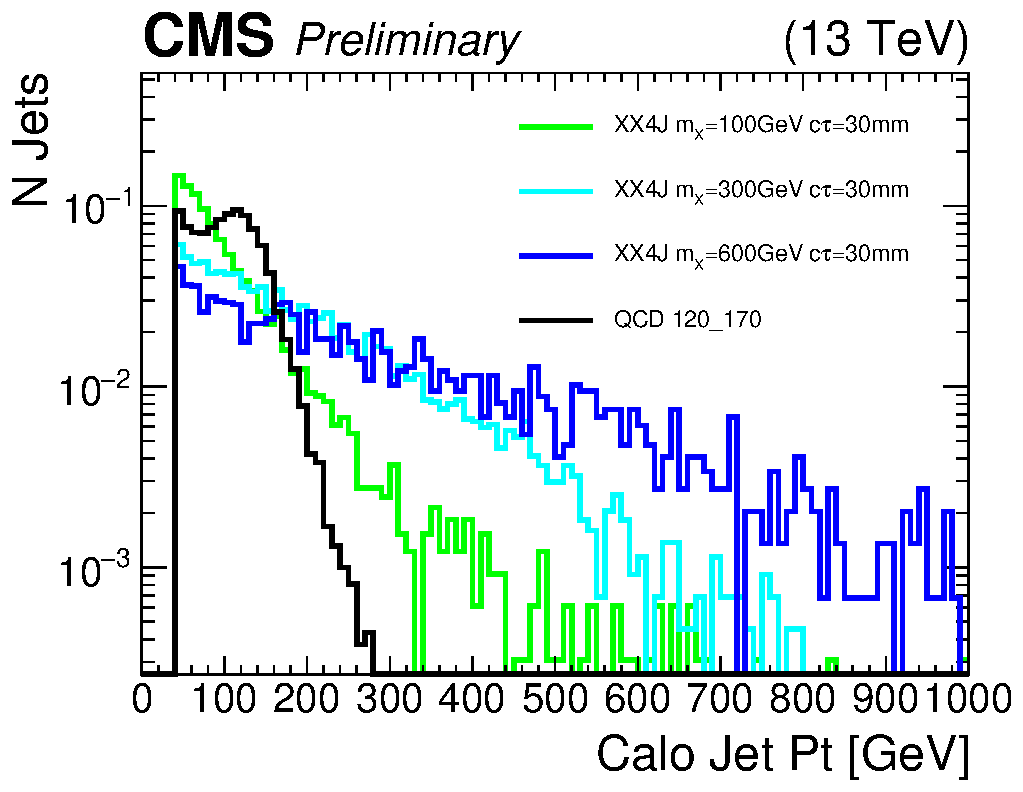
\includegraphics[width=.45\textwidth]{figures/an_jetid/VTX_MATCH_IP/XX4J_MASS_caloJetPt}
%% 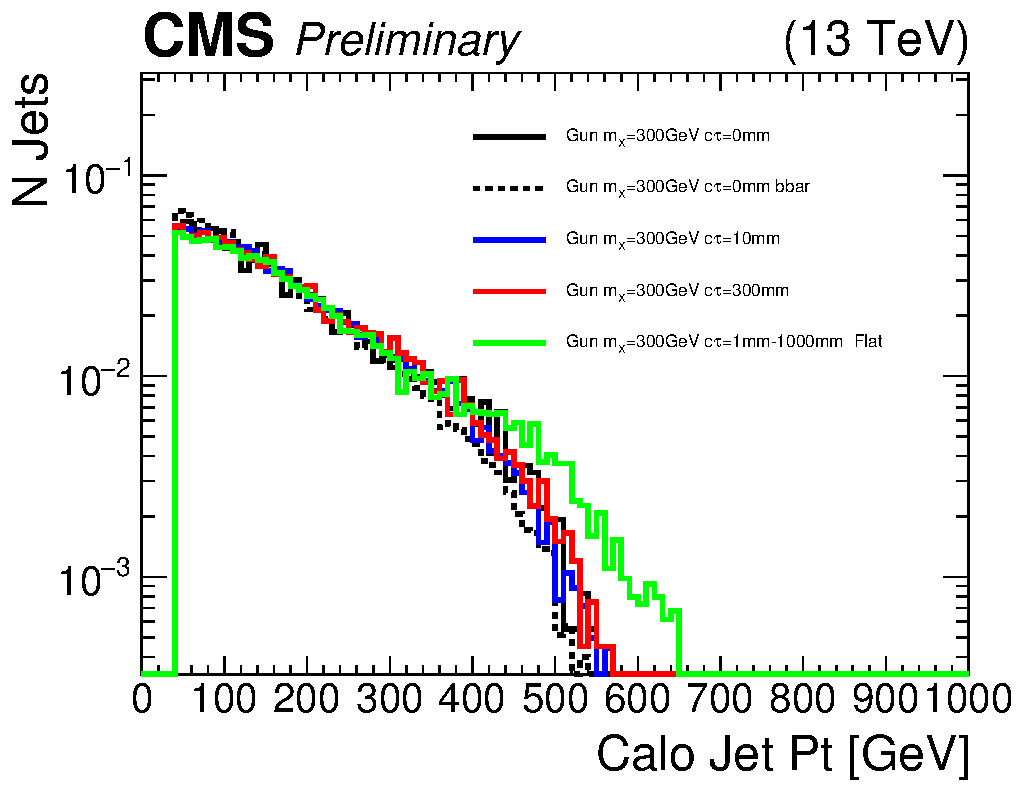
\includegraphics[width=.45\textwidth]{figures/an_jetid/VTX_MATCH_IP/GUN_caloJetPt}
%% \end{center}
%% \caption{The calo jet $p_{t}$ of the $XX4J$ and $GUN$ samples.}
%% \label{fig:xx4j_gun_caloJetPT}
%% \end{figure}

The reconstructed calo jet transverse momentum for varied lifetimes is not especially sensitive to the lifetime of the decaying $X^0$ (Fig. \ref{fig:xx4j_gun_caloJetPT})
until very long lifetimes. The flat lifetime gun sample develops high transverse momentum (relative to the shorter lifetime) jets when the long lived $X^0$ decays at 
a transverse distance far enough from the beamline to be reconstructed as a single jet, or
decaying entirely inside the calorimeter. 


\section{Individual Variable Studies}


\subsection{Impact Parameter Information}

\begin{figure}
\begin{center}
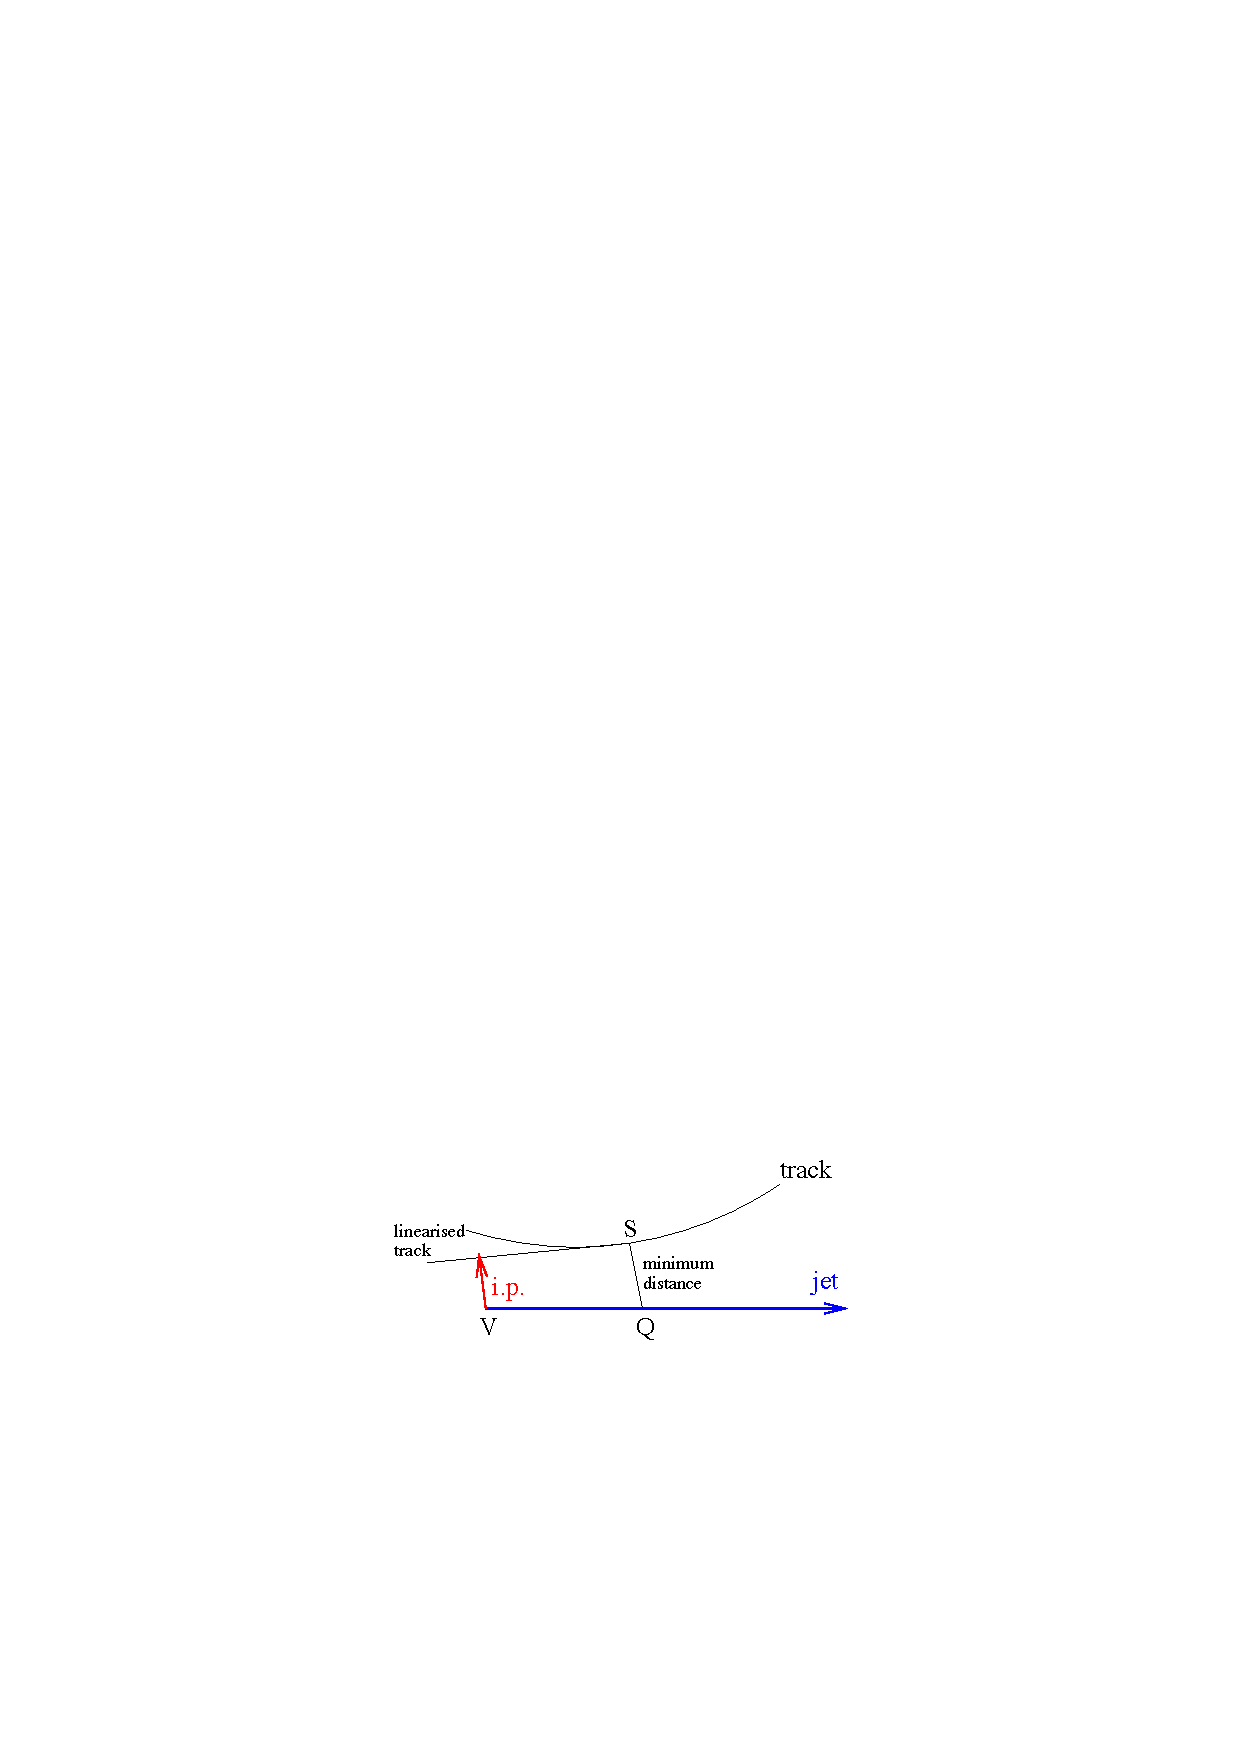
\includegraphics[width=.7\textwidth]{figures/an_jetid/DIAGRAMS/ip_diagram}
\end{center}
\caption{Diagram depicting the impact parameter calculation. $V$ is the position of the primary vertex. $\vec j = \vec{VQ}$ is the direction of 
the calo jet. $S$ is the point on the track extrapolation backward from the inner hit which is closest to the jet axis. From $S$ the track is
linearized and extrapolated backwards. The impact parameter magnitude is the minimal distance on the linearized track from the primary vertex. We
will denote the vector from the primary vertex to the point of minimal distance on the linearized track as $\vec{IP}$}
\label{fig:ipdiagram}
\end{figure}

\begin{figure}
\begin{center}
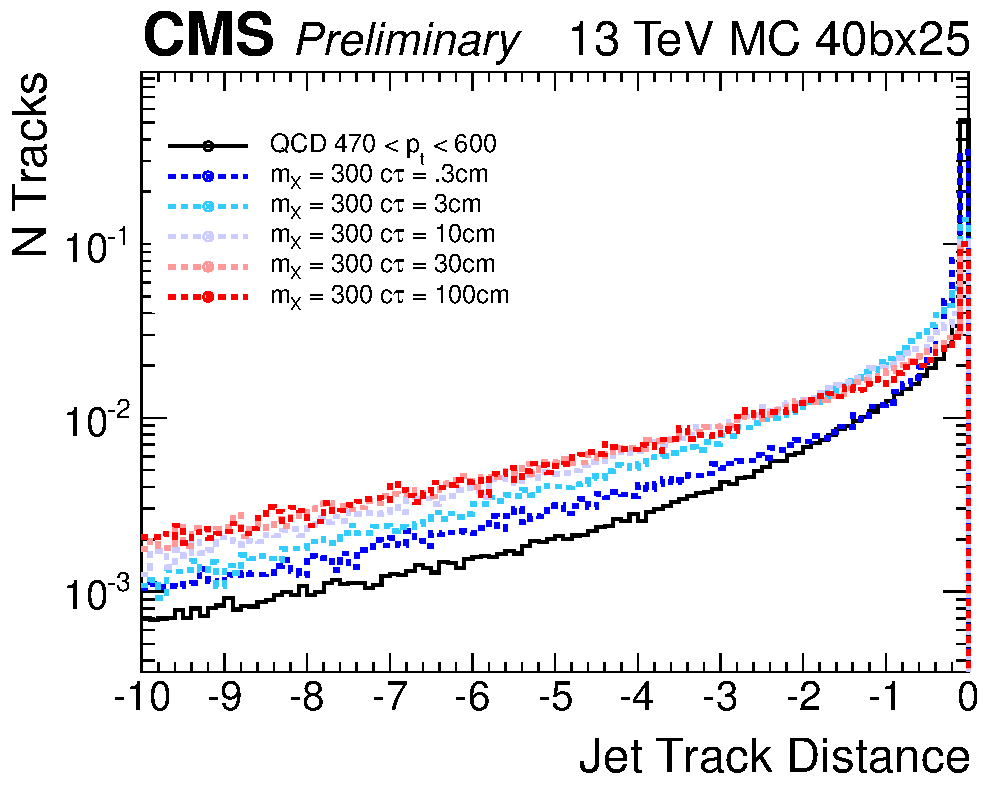
\includegraphics[width=.7\textwidth]{figures/an_jetid/VTX_MATCH_IP/liTrackDistanceJetAxis}
\end{center}
\caption{The closest distance between the jet axis and track}
\label{fig:distance}
\end{figure}

The tracks originating from a decay at a displaced vertex will have large impact parameters relative
to the true primary vertex. The impact parameter is calculated by starting from the particle trajectory at the
innermost measurement point and extrapolating backward to the minimum distance between the track and jet direction $\vec{j}$ (Fig \ref{fig:distance}).
Here, the track is linearized by taking the line tangent to the track at this point. The minimum distance from this linearized
track to the primary vertex gives the magnitude of the impact parameter. We will refer to the vector pointing from the
primary vertex to the point of minimum distance as $\vec{IP}$ (Fig. \ref{fig:ipdiagram}). 


\begin{figure}
\begin{center}
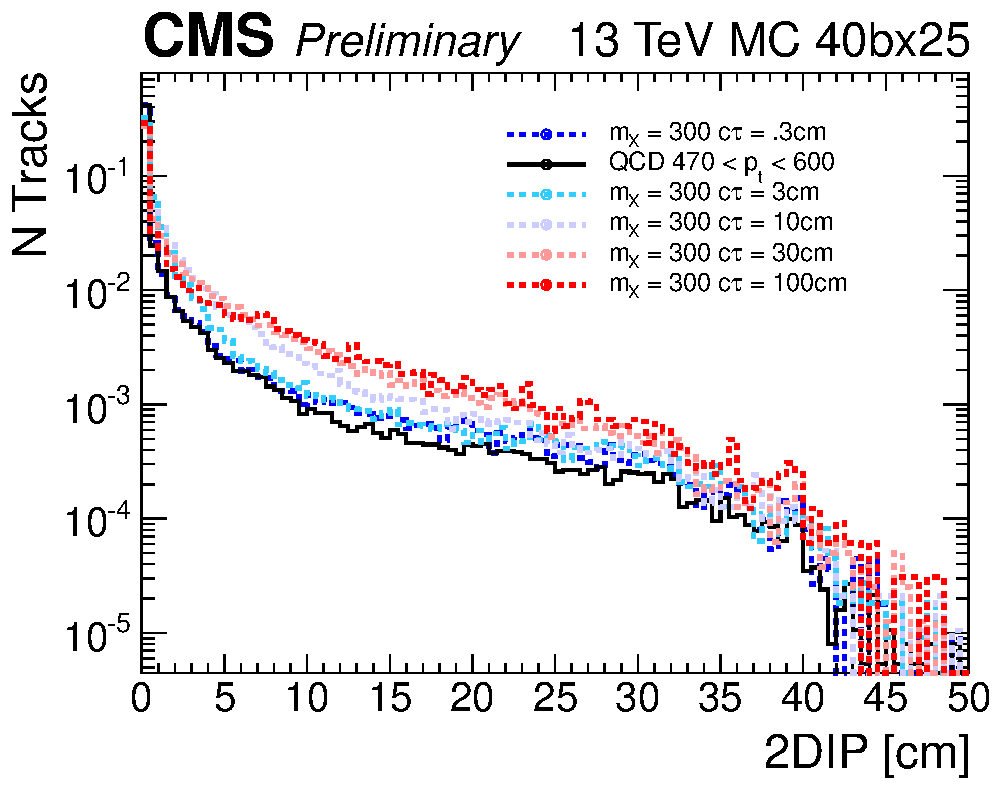
\includegraphics[width=.45\textwidth]{figures/an_jetid/VTX_MATCH_IP/liTrackIP2D}
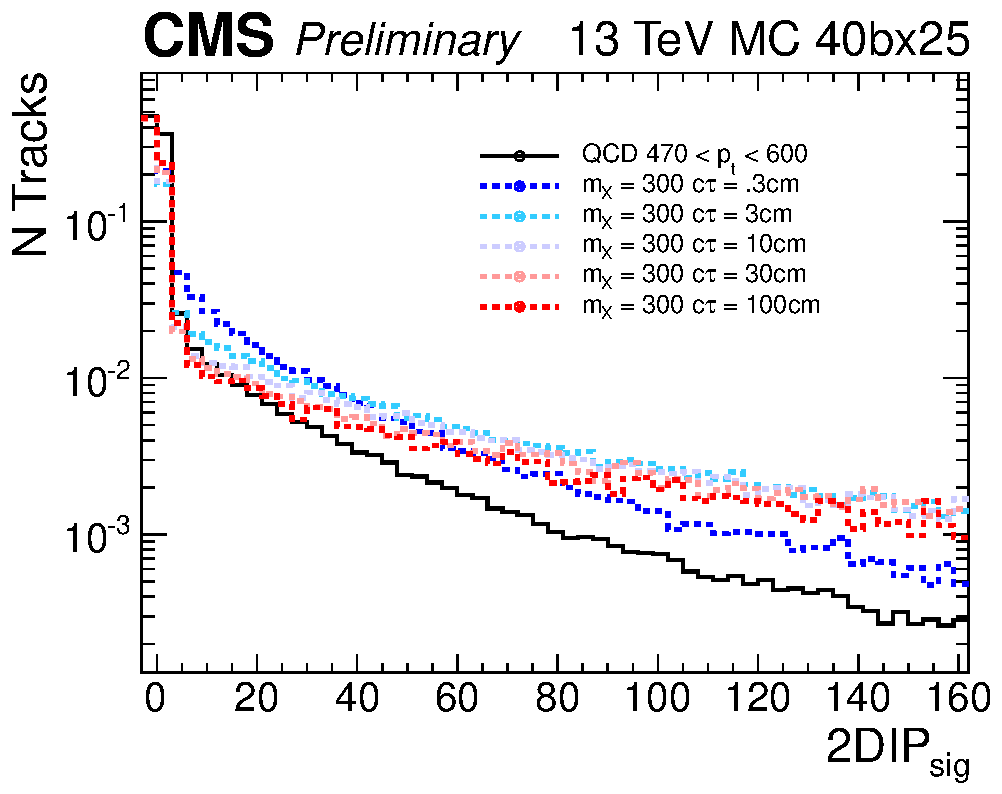
\includegraphics[width=.45\textwidth]{figures/an_jetid/VTX_MATCH_IP/liTrackIPSig2D}\\
\end{center}
\caption{The same samples in Fig \ref{fig:ntrack} are shown. (Left) The 2D impact parameter of tracks matched to calo jets matched to 
generator quarks with $\Delta R < 0.5$. (Right) 2D impact parameter significance of the same tracks. All distributions are normalized to 1.}
\label{fig:iptrack}
\end{figure}

\begin{figure}
\begin{center}
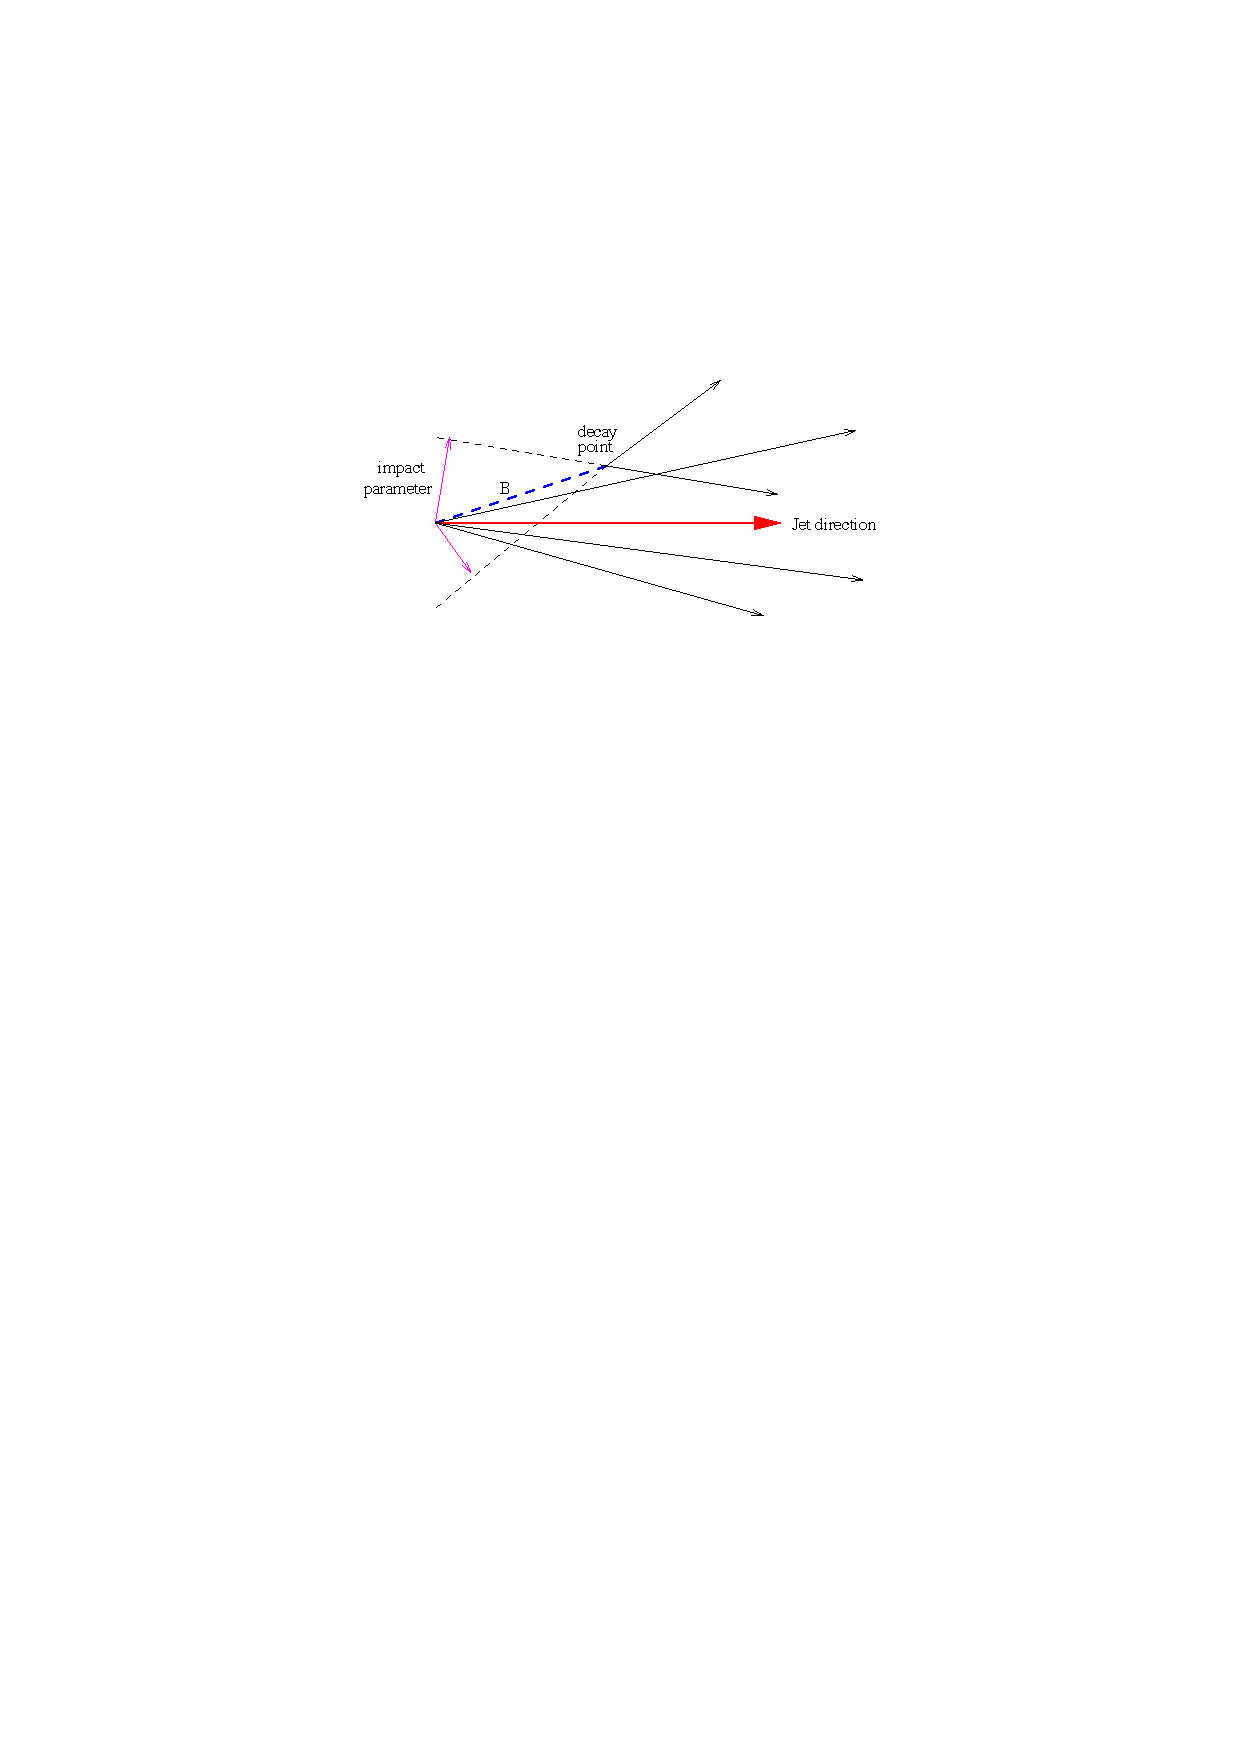
\includegraphics[width=.7\textwidth]{figures/an_jetid/DIAGRAMS/b_diagram}
\end{center}
\caption{Diagram of a B hadron decay showing the mis-alignment of the jet direction from a calo jet and the decay vertex}
\label{fig:bdiagram}
\end{figure}



\begin{figure}
\begin{center}
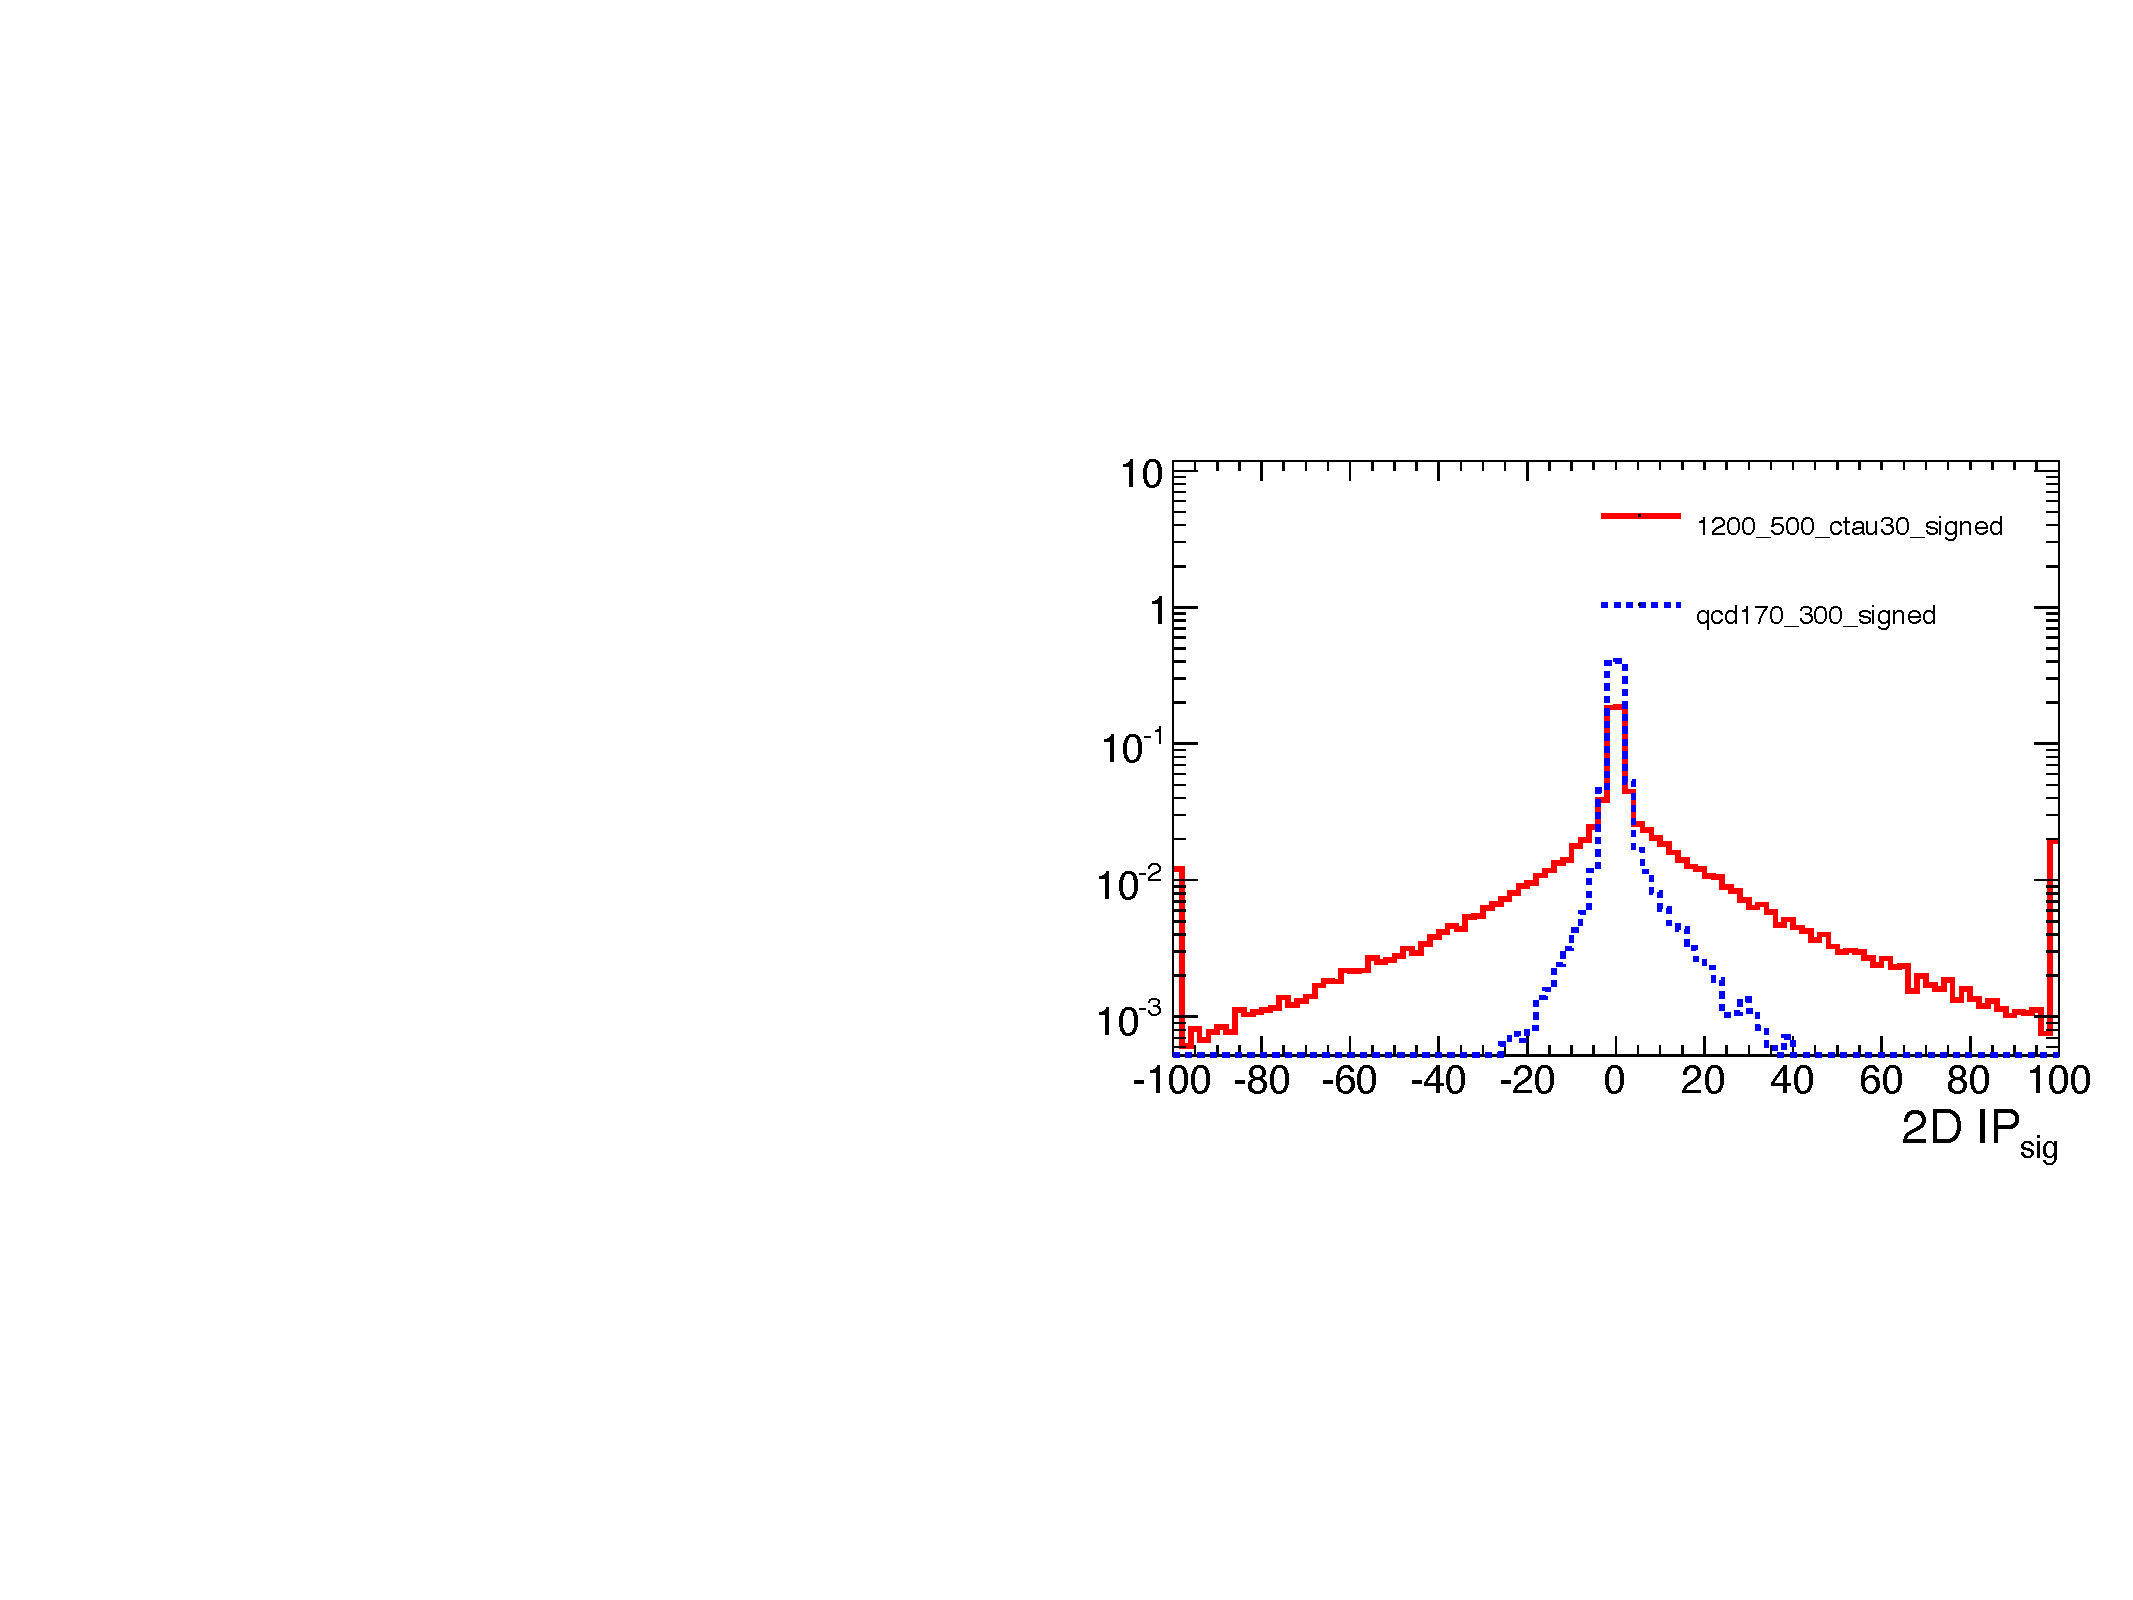
\includegraphics[width=.7\textwidth]{figures/an_jetid/signed_2dipsig}
\end{center}
\caption{Comparison of the $2DIP_{sig}$ of tracks within 1) QCD jets and 2) the less boosted decay of a heavy higgs $H^0=1200 GeV$ decaying to two long lived
$X^{0}$ with $m_{X}=500$GeV. As not all tracks are down stream of long lived flight direction there are tracks with large negative values of $2DIP_{sig}$. The
contribution of $B$ mesons producing tracks with large positive $2DIP_{sig}$  can be sign in the asymmetry of the QCD distribution  }
\label{fig:2dipsig_sign}
\end{figure}


The sign of the impact parameter is given as the sign of the scalar product between $\vec{IP}$ and  the direction of the jet: $\vec{IP} \cdot \vec j$. 
For decays where the calo jet direction is accurately reconstructed, the impact parameter of displaced tracks
will have positive sign, corresponding to the decay occurring down stream of the jet direction. As the accuracy of the jet direction
reconstruction depends on the lifetime of the particle producing the jets (Fig. \ref{fig:bdiagram}), we opt to use un-signed IP significance to 
identify displaced jets (Fig. \ref{fig:iptrack}). In example, a case when the signal has large negative values of $2DIP_{sig}$ is shown in Fig \ref{fig:2dipsig_sign}.
 It is important to note that as most $GUN$ samples (excluding the prompt samples) do not 
have a reconstructed primary vertex, a fake primary vertex with a nominal error is introduced in the calculation. 
This biases the impact parameter significance relative to the $XX4J$.

\begin{figure}
\begin{center}
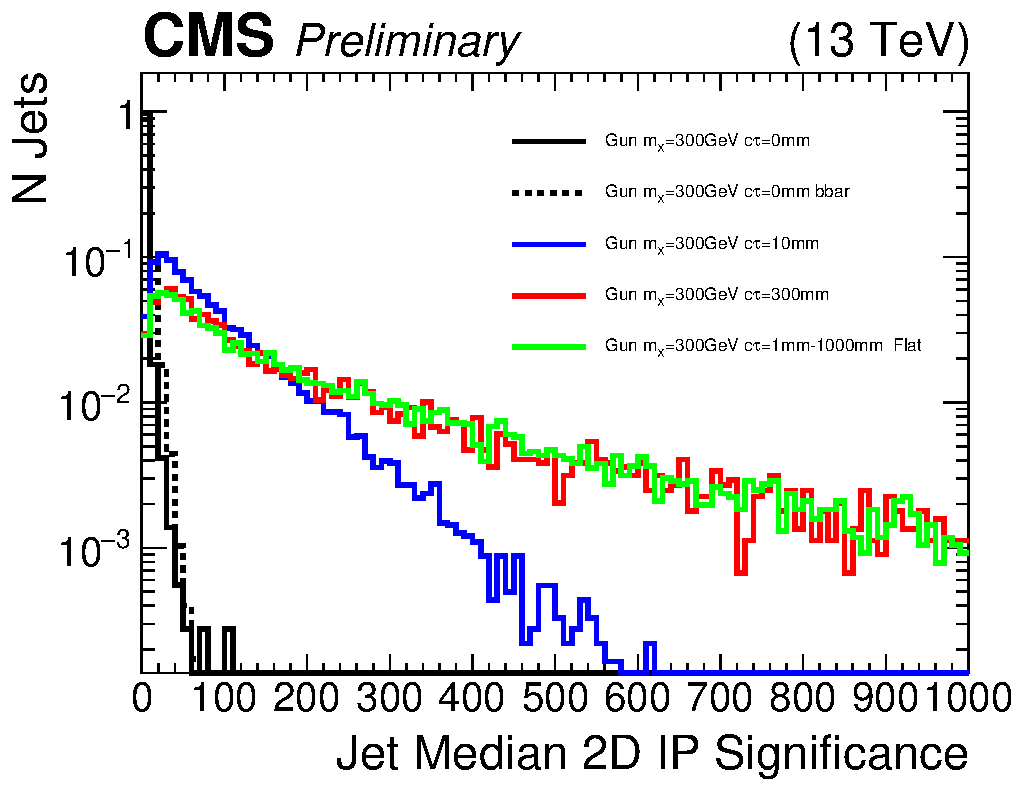
\includegraphics[width=.45\textwidth]{figures/an_jetid/VTX_MATCH_IP/GUN_jetMedianIPSig2D}
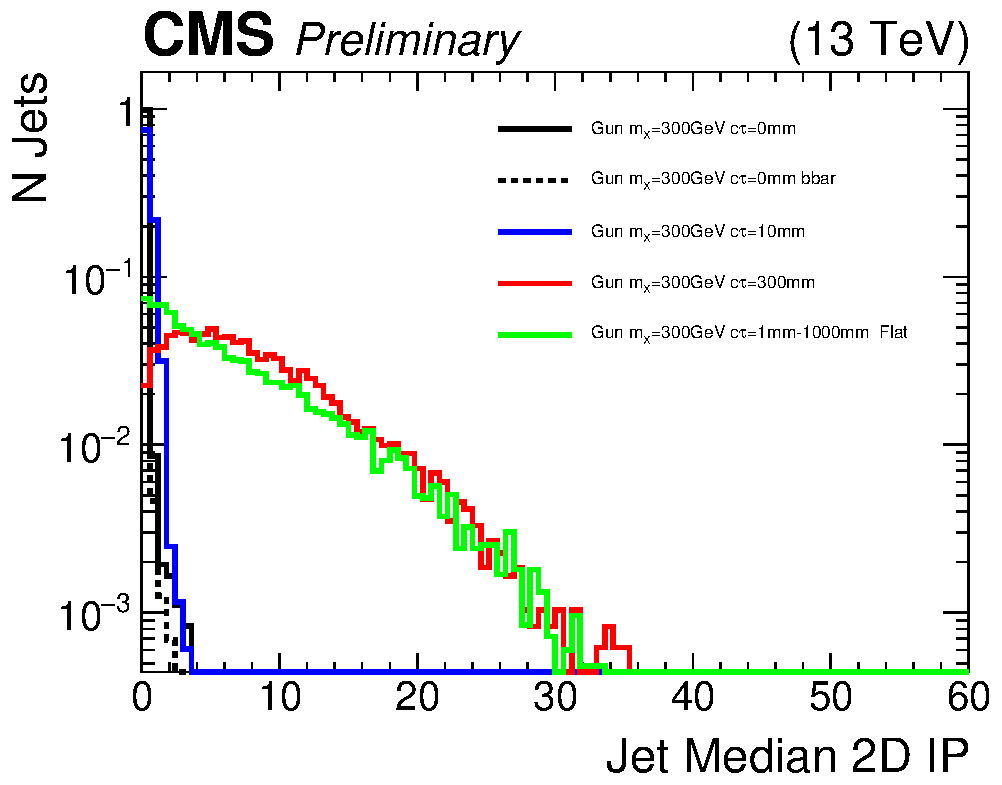
\includegraphics[width=.45\textwidth]{figures/an_jetid/VTX_MATCH_IP/GUN_jetMedianIP2D}
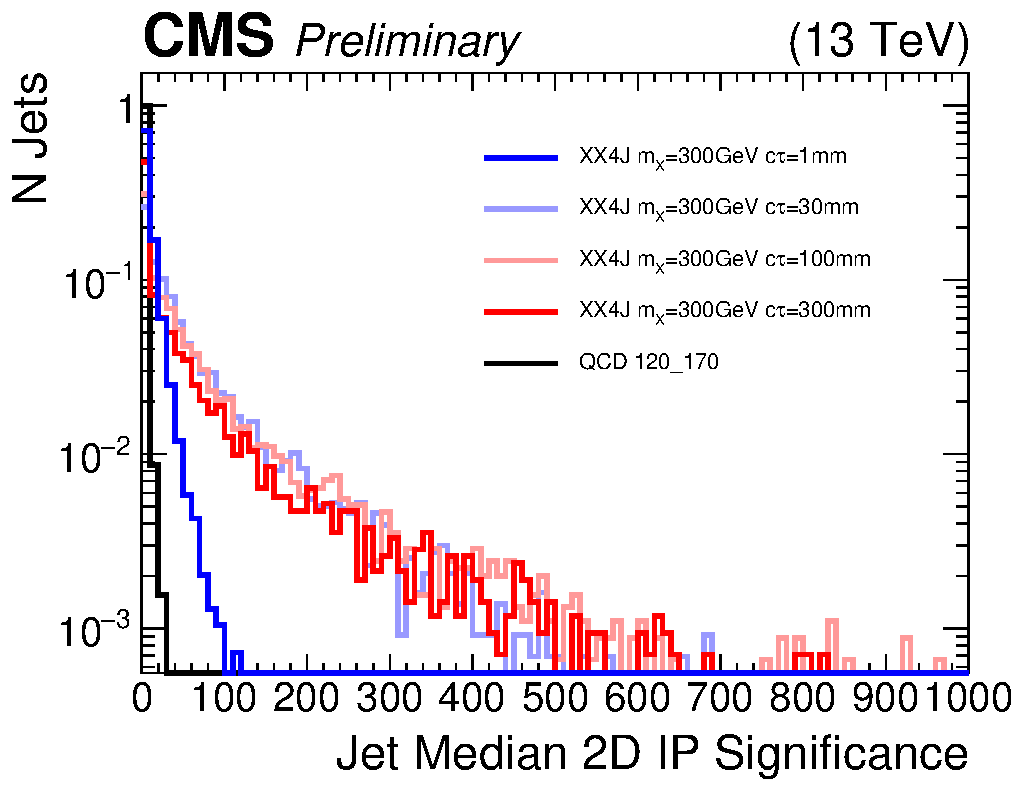
\includegraphics[width=.45\textwidth]{figures/an_jetid/VTX_MATCH_IP/XX4J_jetMedianIPSig2D}
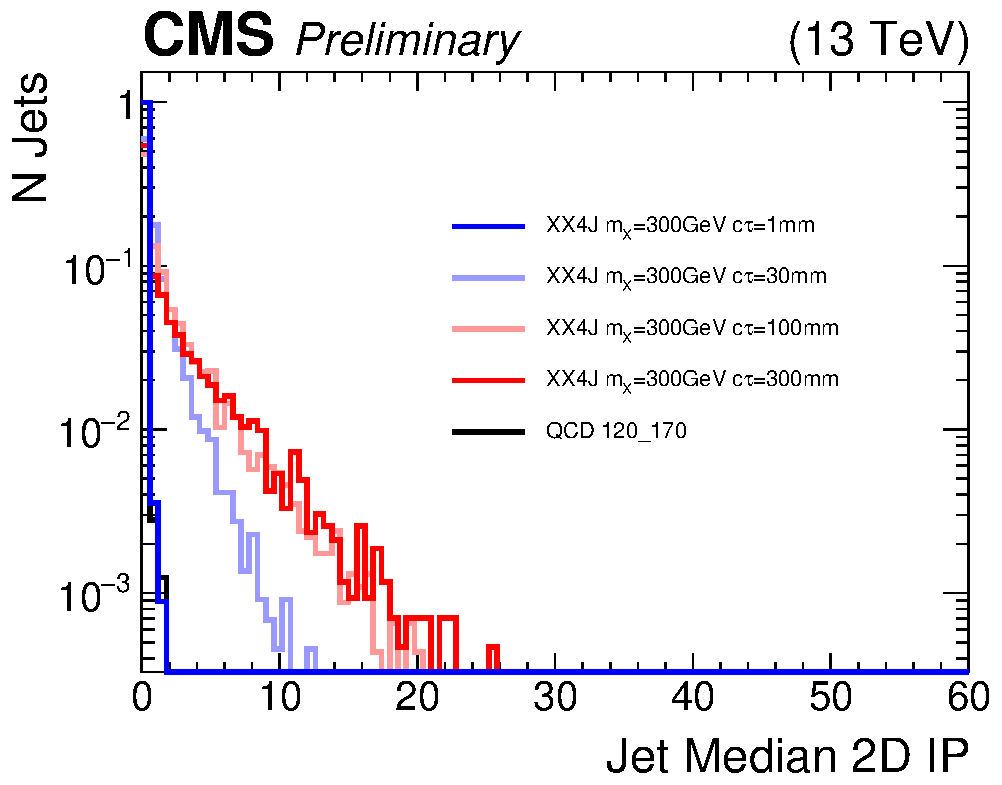
\includegraphics[width=.45\textwidth]{figures/an_jetid/VTX_MATCH_IP/XX4J_jetMedianIP2D}
\end{center}
\caption{Unsigned 2D impact parameter for the $XX4J$ and $GUN$ samples}
\label{fig:ip_vs_ipsig}
\end{figure}

To account for the tracking resolution impact parameter significance is introduced. Tracks with impact
parameter consistent with the primary vertex relative to the tracking resolution given small impact parameter significance $< 5$. 
For decays within $L_{xy} < 10$~mm significance gives significant improvements in signal background separation 
relative to the absolute impact parameter value Fig. \ref{fig:ip_vs_ipsig}.

\begin{figure}
\begin{center}
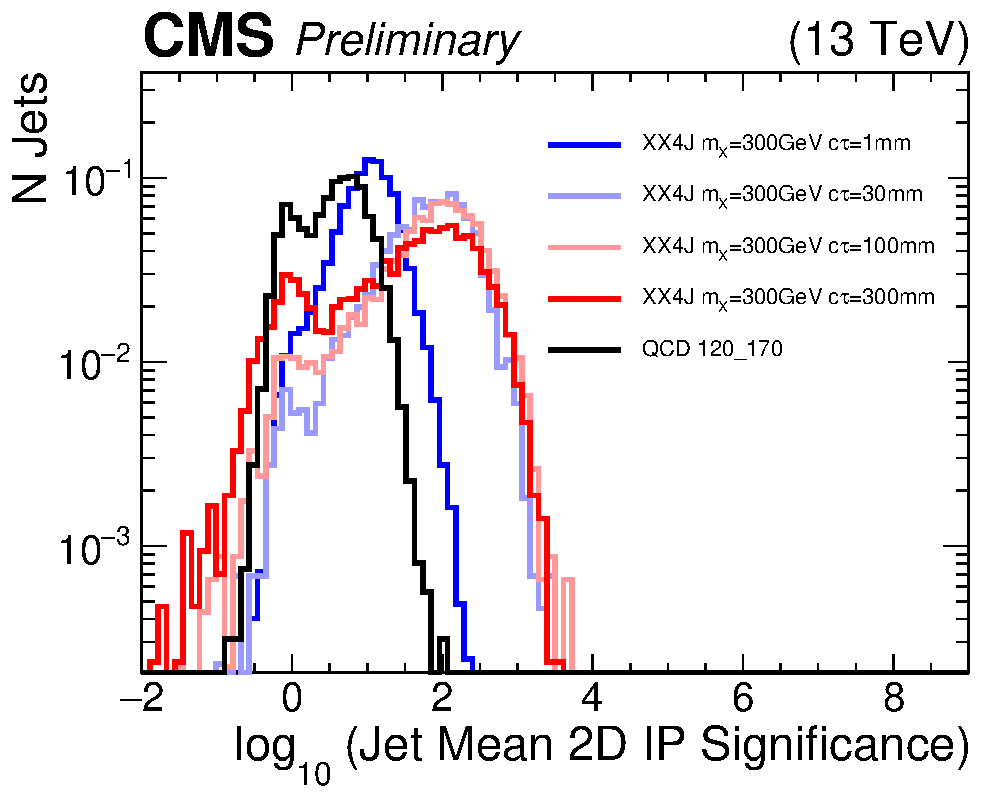
\includegraphics[width=.45\textwidth]{figures/an_jetid/VTX_MATCH_IP/XX4J_log_jetMeanIPSig2D}
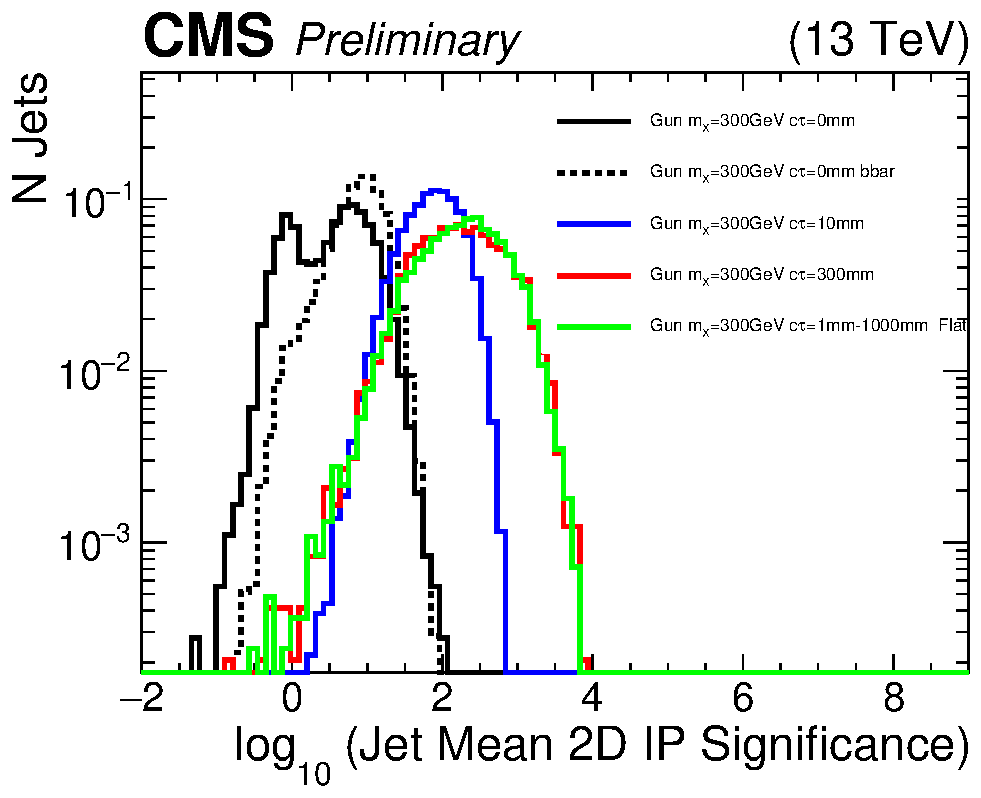
\includegraphics[width=.45\textwidth]{figures/an_jetid/VTX_MATCH_IP/GUN_log_jetMeanIPSig2D}
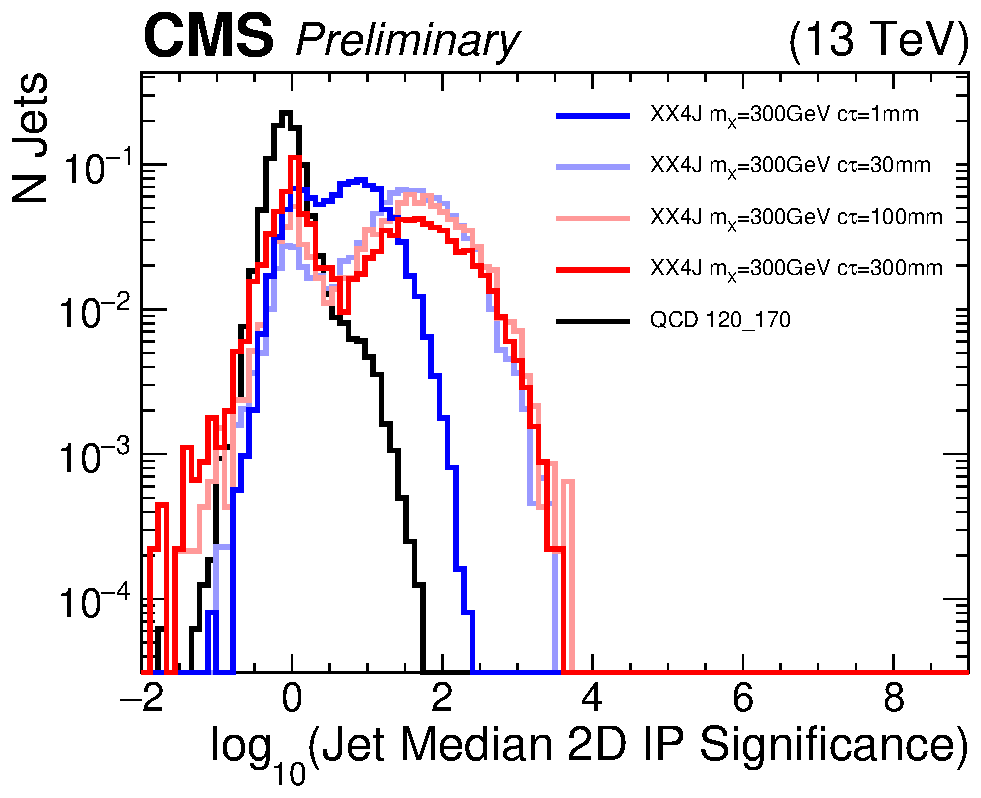
\includegraphics[width=.45\textwidth]{figures/an_jetid/VTX_MATCH_IP/XX4J_log_jetMedianIPSig2D}
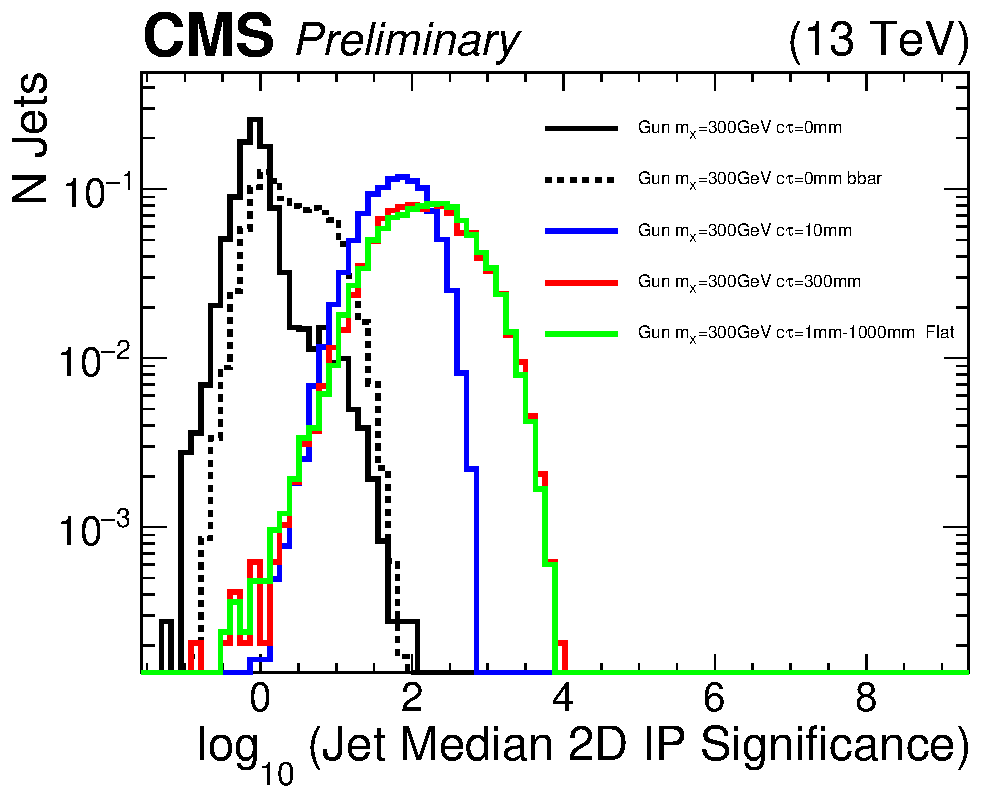
\includegraphics[width=.45\textwidth]{figures/an_jetid/VTX_MATCH_IP/GUN_log_jetMedianIPSig2D}
\end{center}
\caption{A comparison between using mean or median IP significance for the displaced di-jet gun and XX4J signal samples}
\label{fig:ipsig_mean_median}
\end{figure}

Impact parameter tag info is reconstructed with limited requirements on the tracks. No maximum longitudinal or transverse impact parameter
is enforced. No requirement on the number of hits, pixel tracks, or track quality is is required at this step. A maximum $\chi^2 < 20$ of 
the track fit is enforced and a $p_{t}>$ 1 GeV to ensure the track would reach the calorimeter. 

%% \begin{verbatim}
%% displacedLifetimeTagInfos = cms.EDProducer( "TrackIPProducer",
%%     maximumTransverseImpactParameter = cms.double( 999999.0 ),
%%     minimumNumberOfHits = cms.int32( 0 ), 
%%     minimumTransverseMomentum = cms.double( 1.0 ),
%%     primaryVertex = cms.InputTag( 'offlinePrimaryVerticesWithBS'),
%%     maximumLongitudinalImpactParameter = cms.double( 999999.0 ), 
%%     computeGhostTrack = cms.bool( False ),
%%     ghostTrackPriorDeltaR = cms.double( 0.03 ),
%%     jetTracks = cms.InputTag( "displacedAk4JetTracksAssociatorAtVertex" ), 
%%     jetDirectionUsingGhostTrack = cms.bool( False ),
%%     minimumNumberOfPixelHits = cms.int32( 0 ), 
%%     jetDirectionUsingTracks = cms.bool( False ),
%%     computeProbabilities = cms.bool( False ),
%%     useTrackQuality = cms.bool( False ),
%%     maximumChiSquared = cms.double( 20.0 )
%% )
%% \end{verbatim}

Variables leveraging the impact parameter information for a given jet are derived from the distribution of impact parameter significances. 
Fig. \ref{fig:ipsig_mean_median} demonstrates the improved  separation of median IP significance relative
 to the mean (Fig. \ref{fig:ipsig_mean_median}). 
As background QCD jets contain real displaced tracks (Tab. \ref{tab:mesons}, \ref{tab:baryons}), the mean calculation is sensitive
 to outlier tracks with large IP significance. For truly displaced jets, all tracks have large impact parameter preserving 
a high median value. 

\begin{figure}
\begin{center}
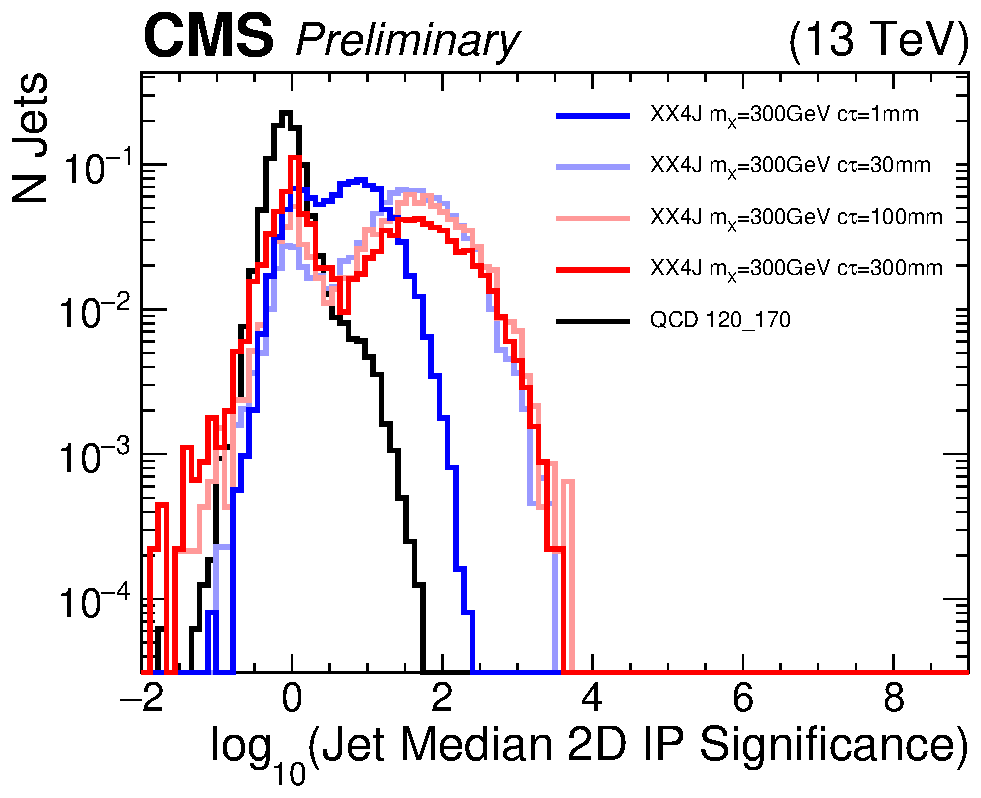
\includegraphics[width=.45\textwidth]{figures/an_jetid/VTX_MATCH_IP/XX4J_log_jetMedianIPSig2D}
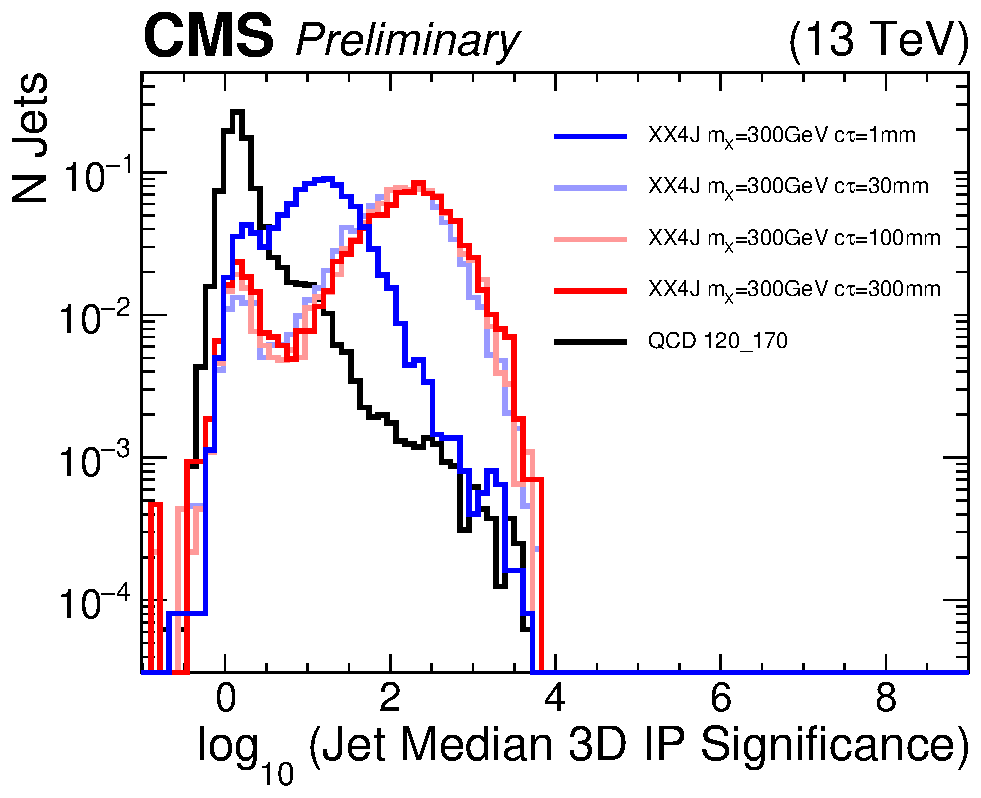
\includegraphics[width=.45\textwidth]{figures/an_jetid/VTX_MATCH_IP/XX4J_log_jetMedianIPSig3D}
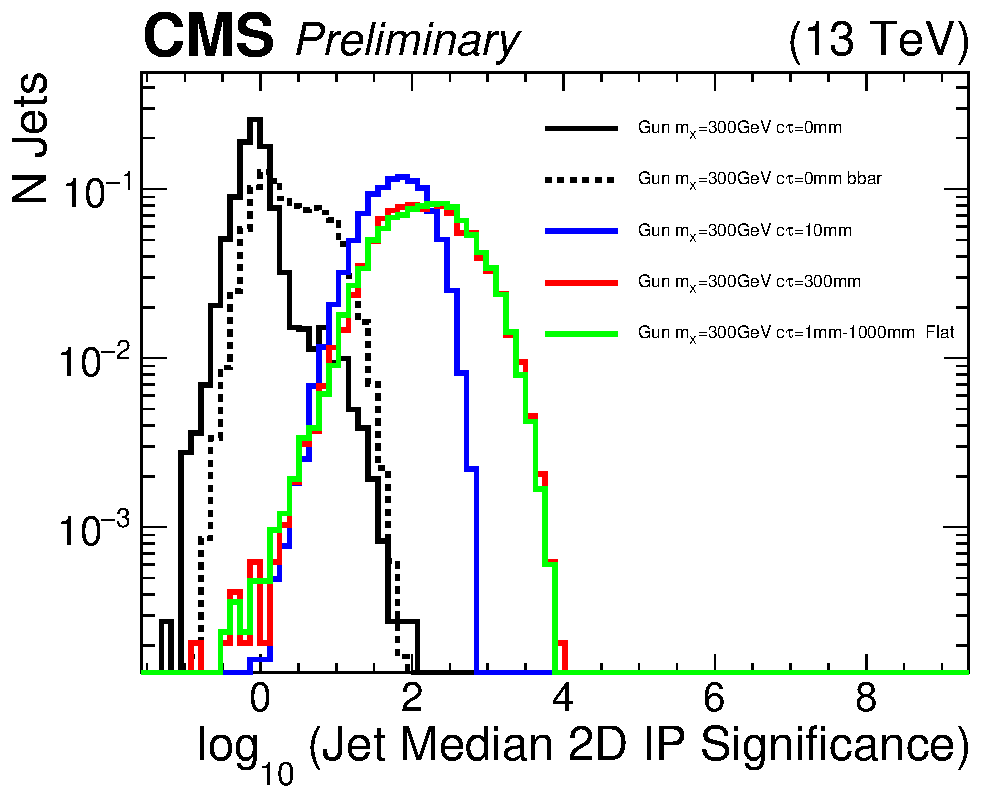
\includegraphics[width=.45\textwidth]{figures/an_jetid/VTX_MATCH_IP/GUN_log_jetMedianIPSig2D}
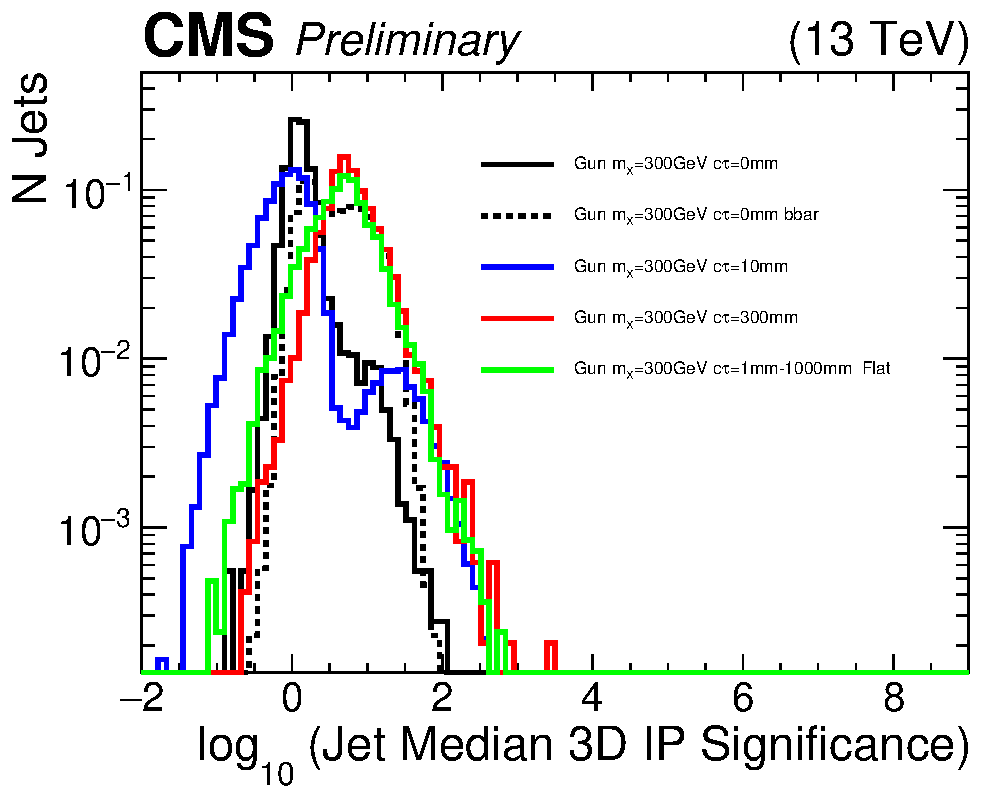
\includegraphics[width=.45\textwidth]{figures/an_jetid/VTX_MATCH_IP/GUN_log_jetMedianIPSig3D}
\end{center}
\caption{A comparison between the median IP Significance in 2D vs 3D for the displaced di-jet gun and  XX4J signal samples}
\label{fig:ipsig_2d_3d}
\end{figure}

The tracks from displaced jets should not have significant contribution from tracks included in a primary vertex. This reduces the likelihood of selecting the correct
primary vertex for the calculation of 3D impact parameters. Instead, we opt to use exclusively transverse quantities that depend only loosely
on the primary vertex selection when a beam-spot constraint is applied.  Fig. \ref{fig:ipsig_2d_3d} shows the comparison between the 2D and 3D
impact parameters showing greater separation for using traverse impact parameters. For the displaced di-jet gun samples, a primary vertex
is rarely reconstructed for longer lifetimes. In this case, a fake PV is built and the resulting discrimination power is lost in the longitudinal
axis. 

\begin{figure}
\begin{center}
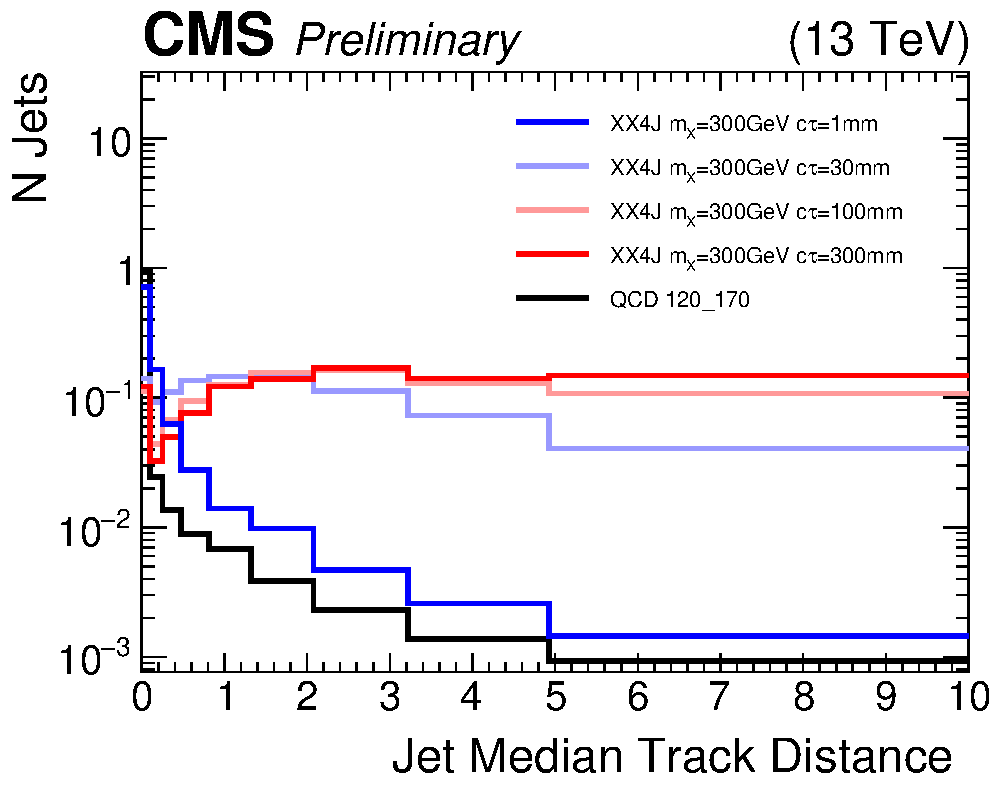
\includegraphics[width=.45\textwidth]{figures/an_jetid/VTX_MATCH_IP/XX4J_jetMedianDistance}
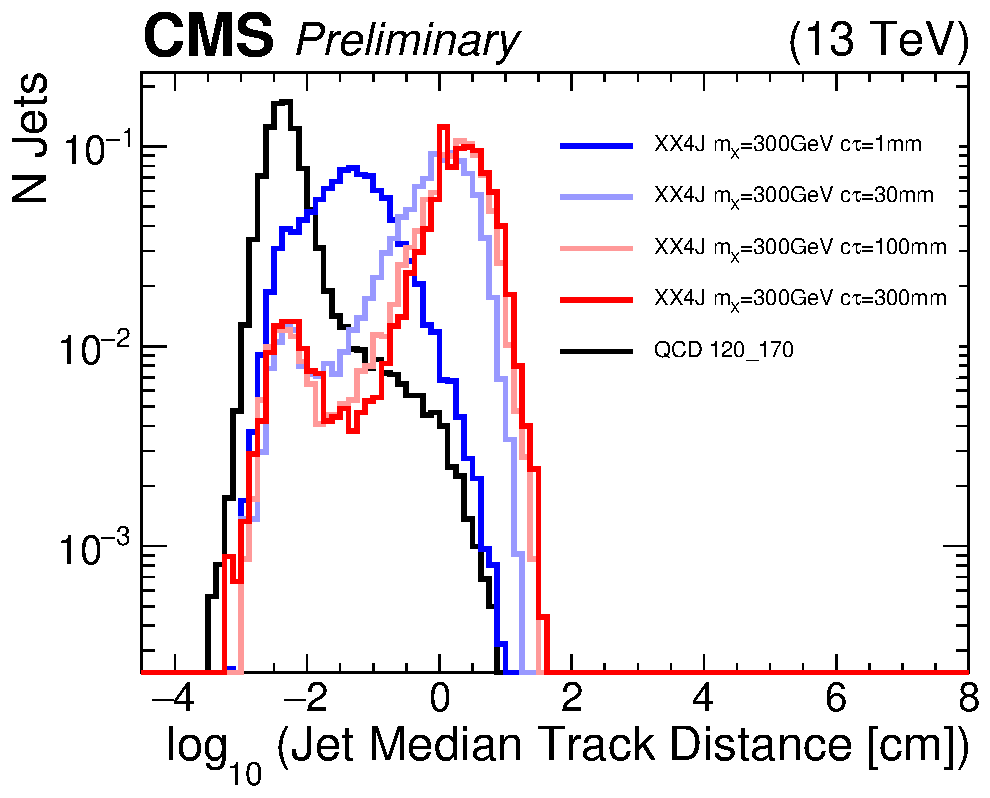
\includegraphics[width=.45\textwidth]{figures/an_jetid/VTX_MATCH_IP/XX4J_log_jetMedianTrackDist}
\end{center}
\caption{For each track in a jet the minimum distance between the track and the jet axis is computed. From this distrubtion
the median is computed for each jet.}
\label{fig:jetDistance}
\end{figure}


\begin{figure}
\begin{center}
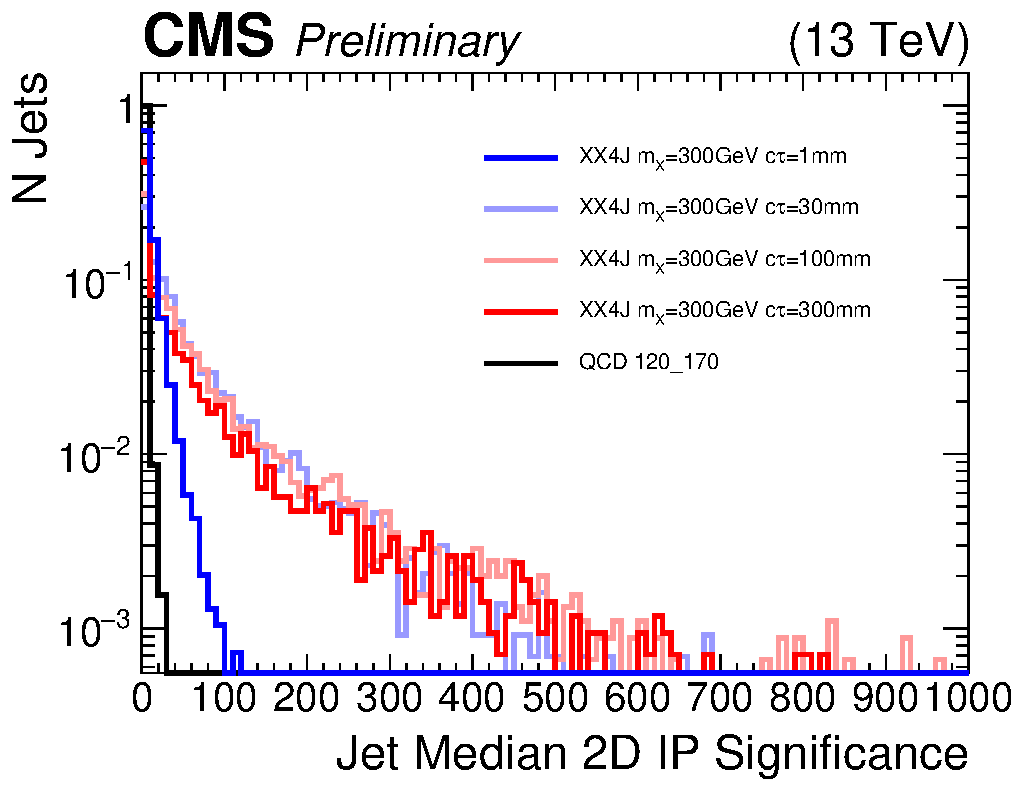
\includegraphics[width=.45\textwidth]{figures/an_jetid/VTX_MATCH_IP/XX4J_jetMedianIPSig2D}
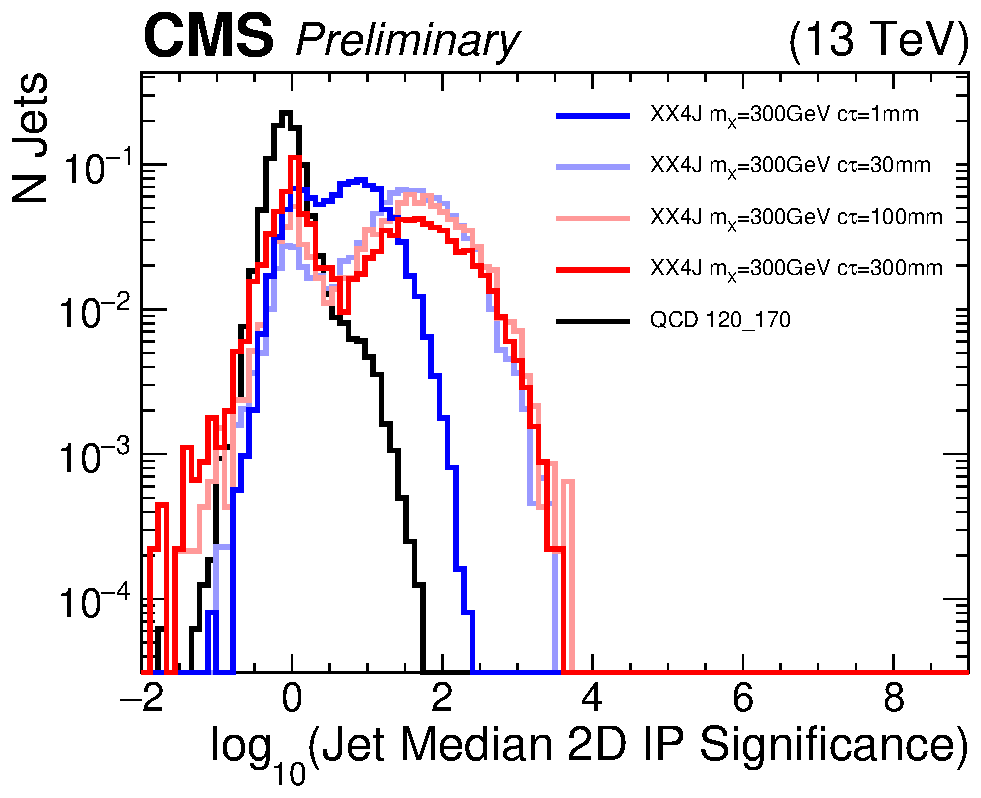
\includegraphics[width=.45\textwidth]{figures/an_jetid/VTX_MATCH_IP/XX4J_log_jetMedianIPSig2D}
\end{center}
\caption{A comparison between log and linear scale variables. The log scale case shows the distinct population
of significances related to pileup in the $XX4J$ sample.}
\label{fig:xx4j_iptrack}
\end{figure}


\begin{figure}
\begin{center}
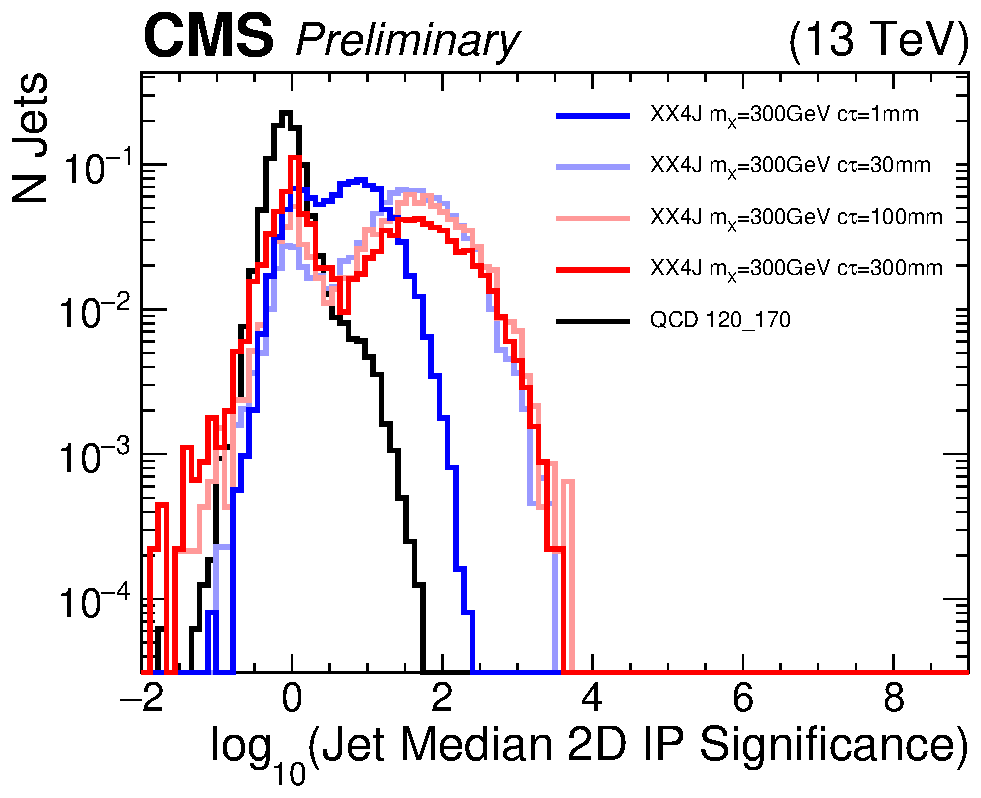
\includegraphics[width=.45\textwidth]{figures/an_jetid/VTX_MATCH_IP/XX4J_log_jetMedianIPSig2D}
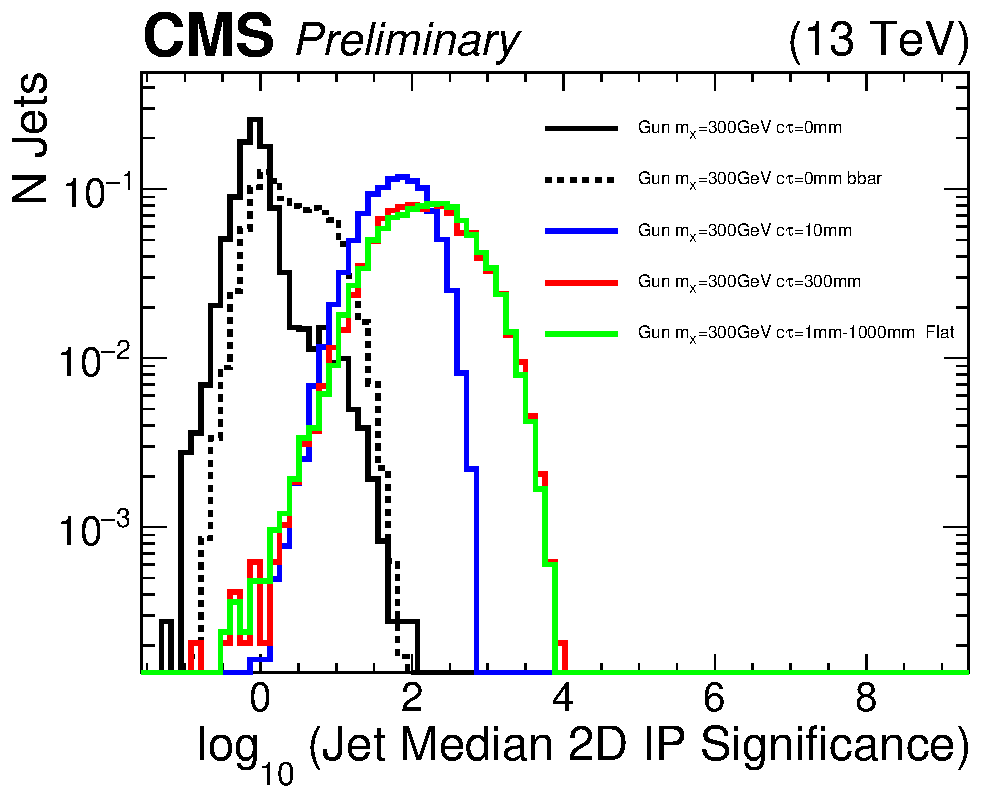
\includegraphics[width=.45\textwidth]{figures/an_jetid/VTX_MATCH_IP/GUN_log_jetMedianIPSig2D}
\end{center}
\caption{A comparison of the Jet Median 2D IP significance between the displaced di-jet gun and XX4J samples}
\label{fig:gun_ipsig}
\end{figure}



\begin{figure}
\begin{center}
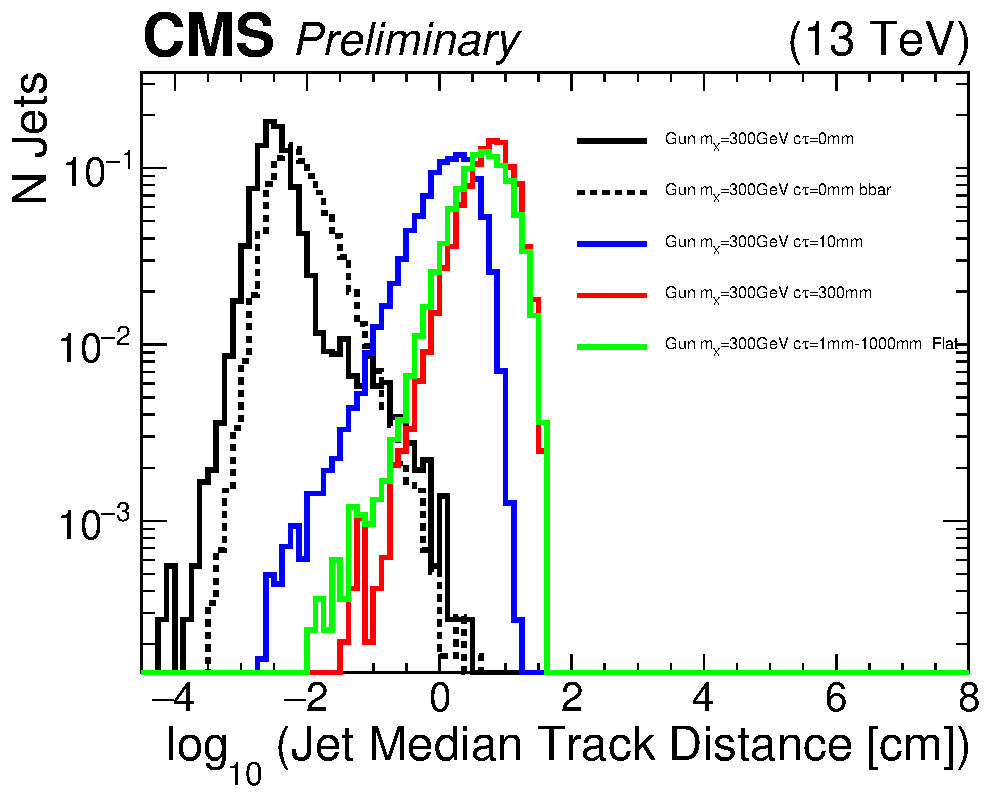
\includegraphics[width=.45\textwidth]{figures/an_jetid/VTX_MATCH_IP/GUN_log_jetMedianTrackDist}
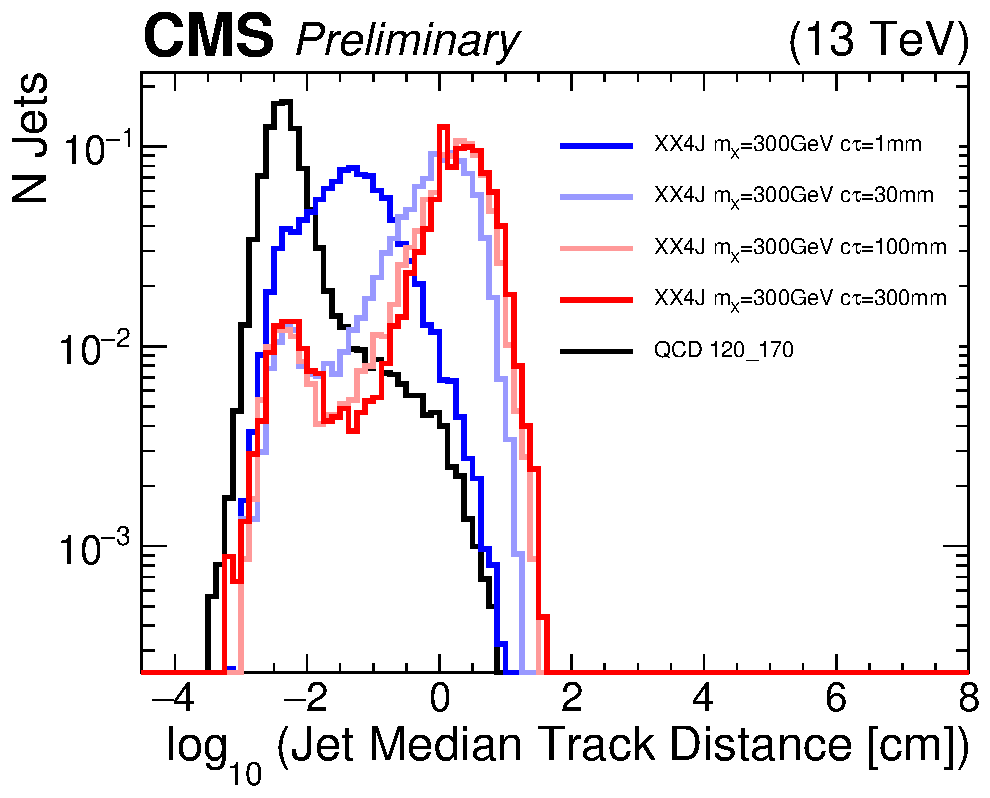
\includegraphics[width=.45\textwidth]{figures/an_jetid/VTX_MATCH_IP/XX4J_log_jetMedianTrackDist}
\end{center}
\caption{The closest distance between the jet axis and track}
\label{fig:jetDist}
\end{figure}


\begin{figure}
\begin{center}
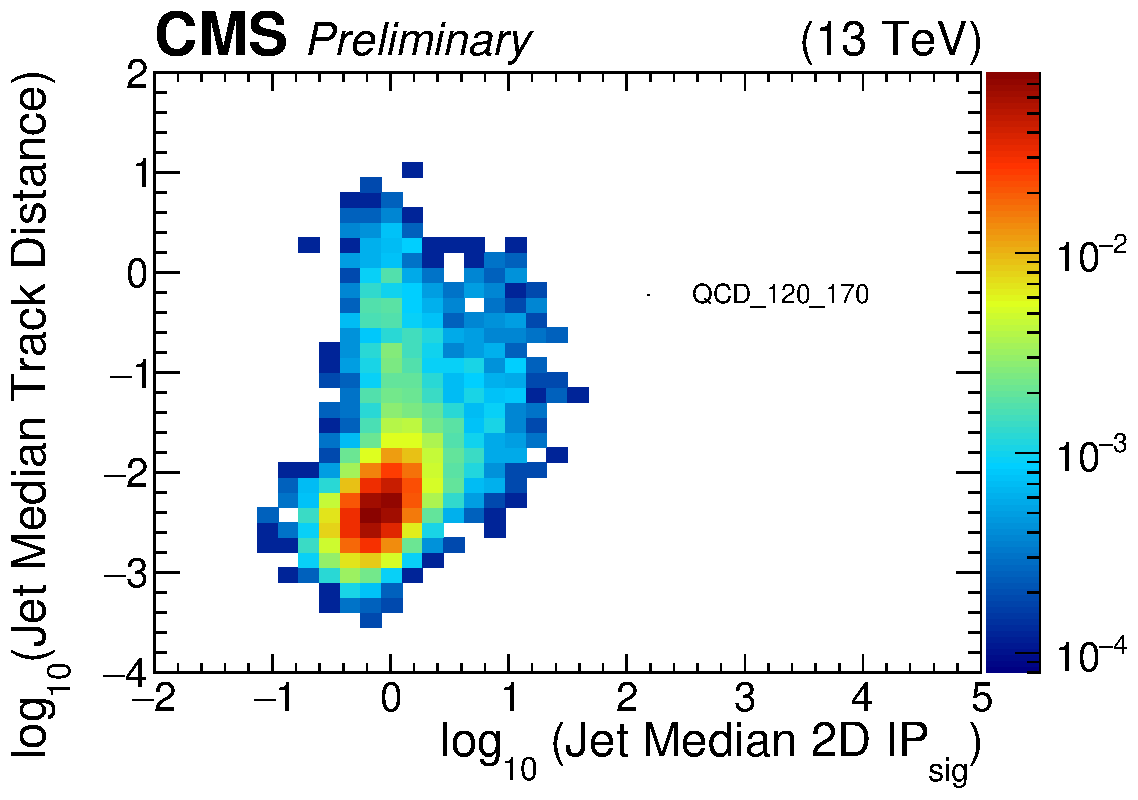
\includegraphics[width=.45\textwidth]{figures/an_jetid/VTX_MATCH_IP/QCD_2D_ipsig_jetDist}
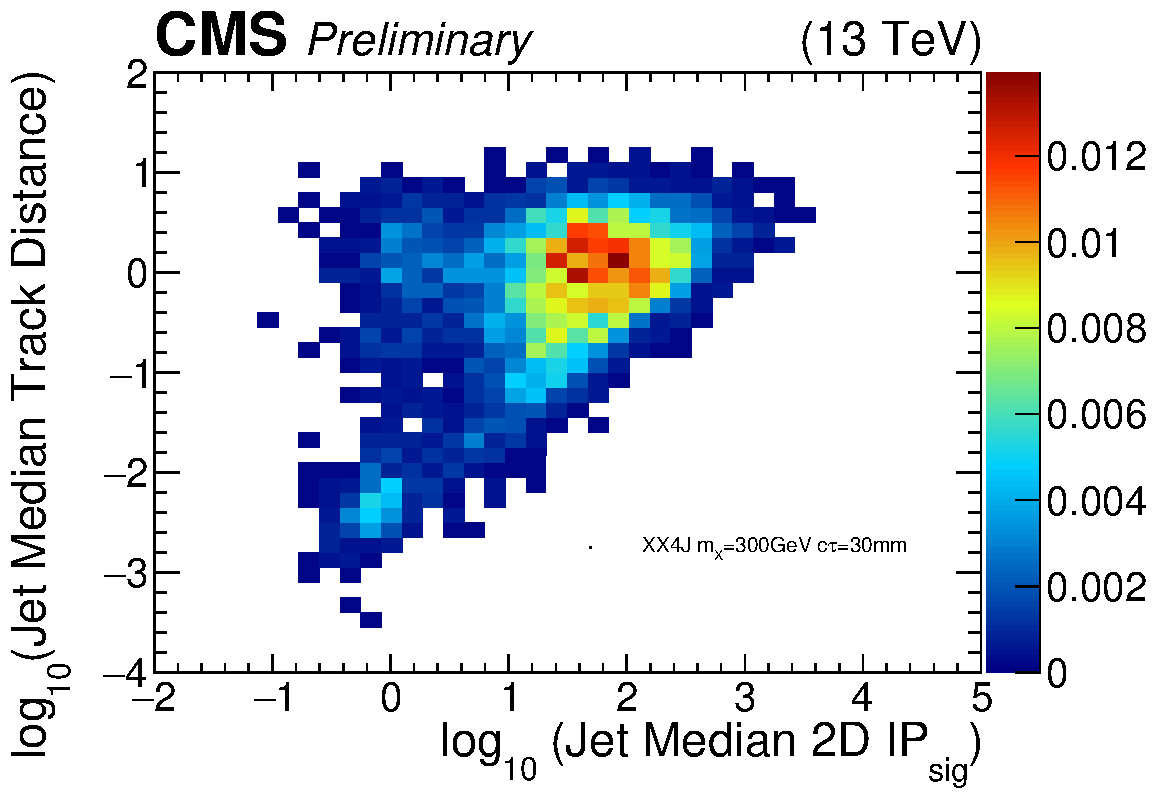
\includegraphics[width=.45\textwidth]{figures/an_jetid/VTX_MATCH_IP/XX4J_2D_ipsig_jetDist}
\end{center}
\caption{Correlations between the IP significance and the jet distance variables}
\label{fig:jetDist_ipsig}
\end{figure}

\subsubsection{Jet Primary Vertex Fraction (Alpha and Beta)}

\begin{figure}
\begin{center}
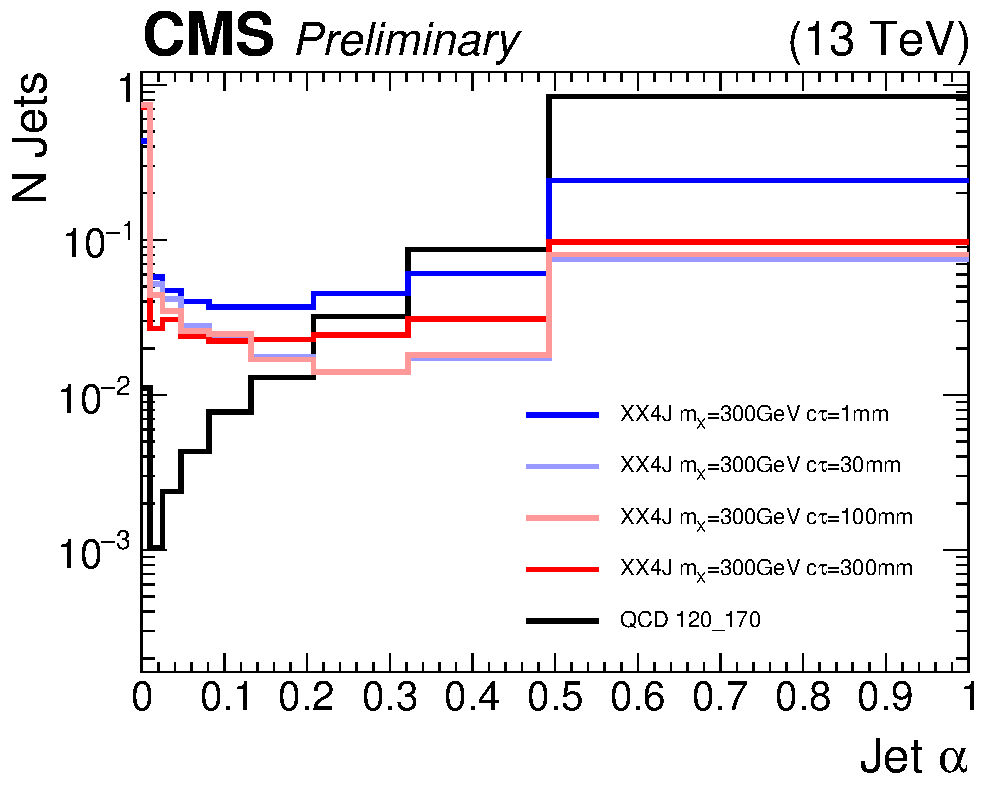
\includegraphics[width=.45\textwidth]{figures/an_jetid/VTX_MATCH_IP/XX4J_alpha}
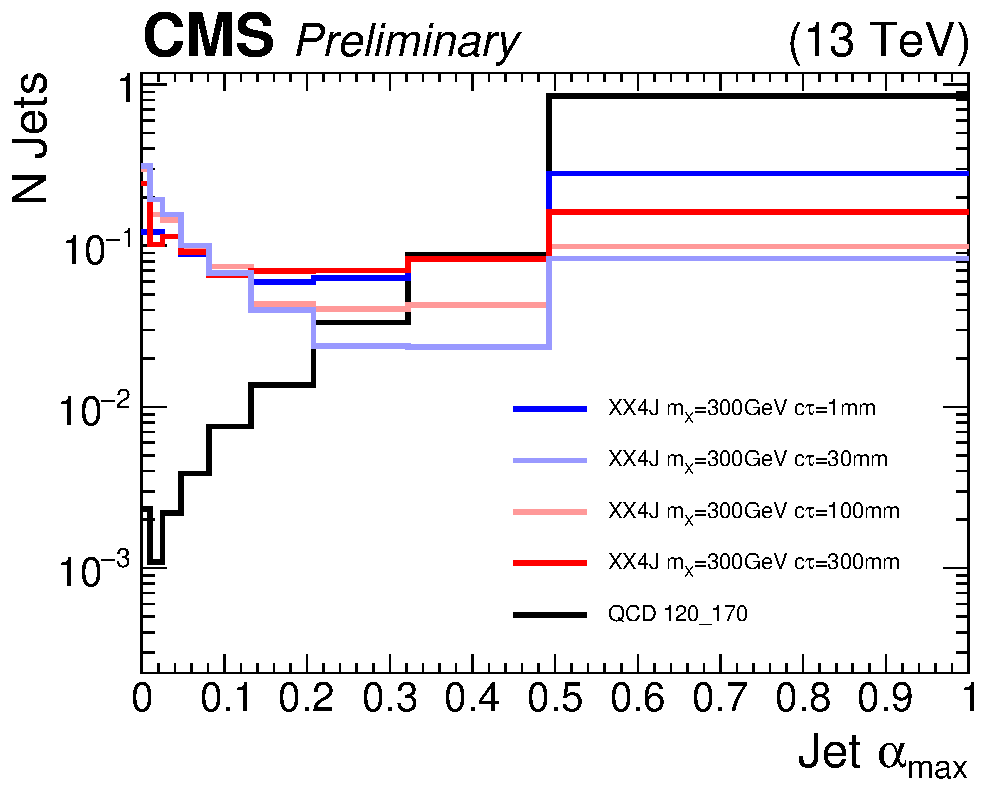
\includegraphics[width=.45\textwidth]{figures/an_jetid/VTX_MATCH_IP/XX4J_alphaMax}
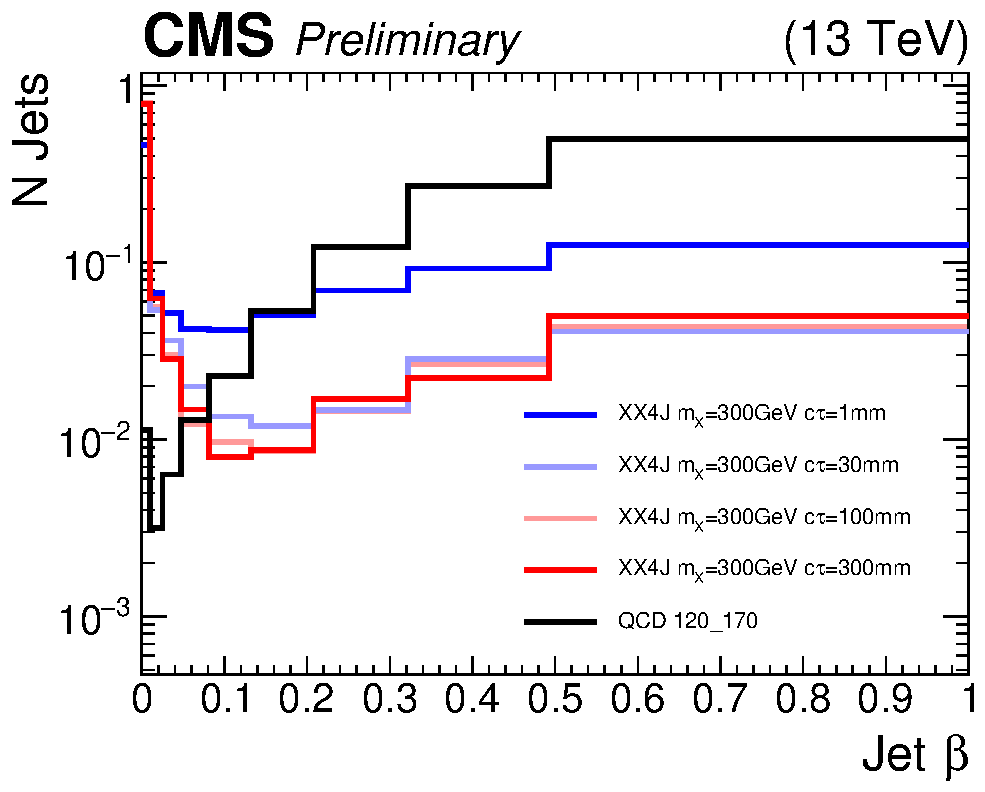
\includegraphics[width=.45\textwidth]{figures/an_jetid/VTX_MATCH_IP/XX4J_beta}
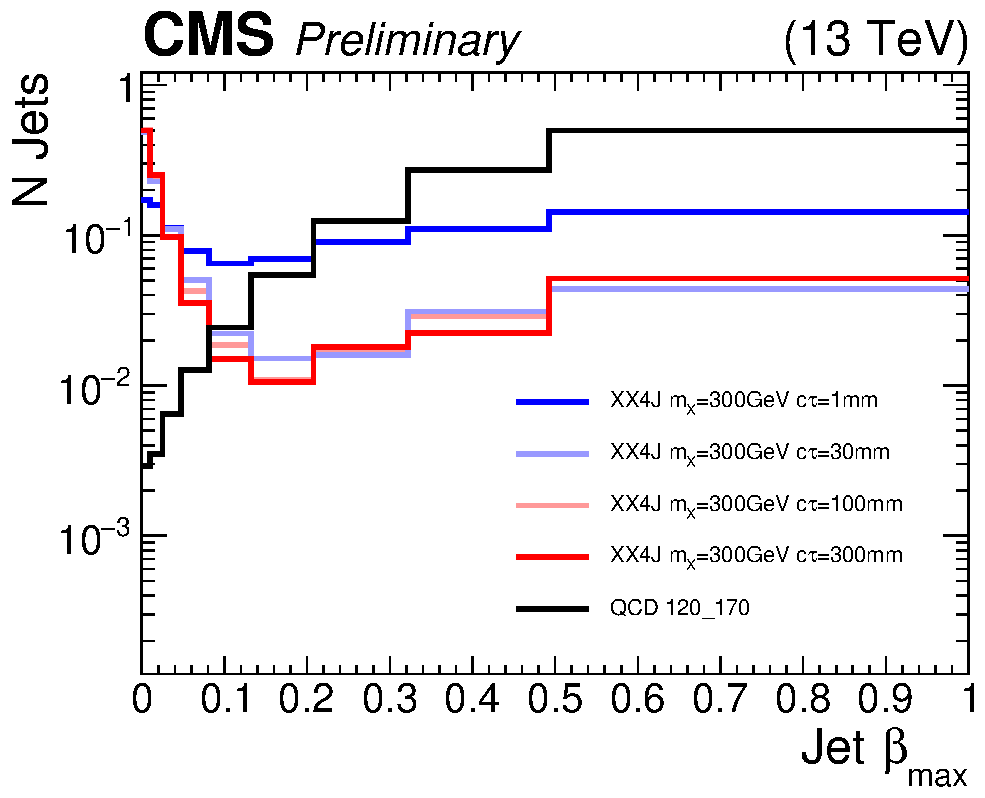
\includegraphics[width=.45\textwidth]{figures/an_jetid/VTX_MATCH_IP/XX4J_betaMax}
\end{center}
\caption{$\alpha, \alpha_{max}, \beta, \beta_{max}$ when varying the lifetime of the decaying $X^0$}
\label{fig:xx4j_alpha_beta}
\end{figure}

\begin{figure}
\begin{center}
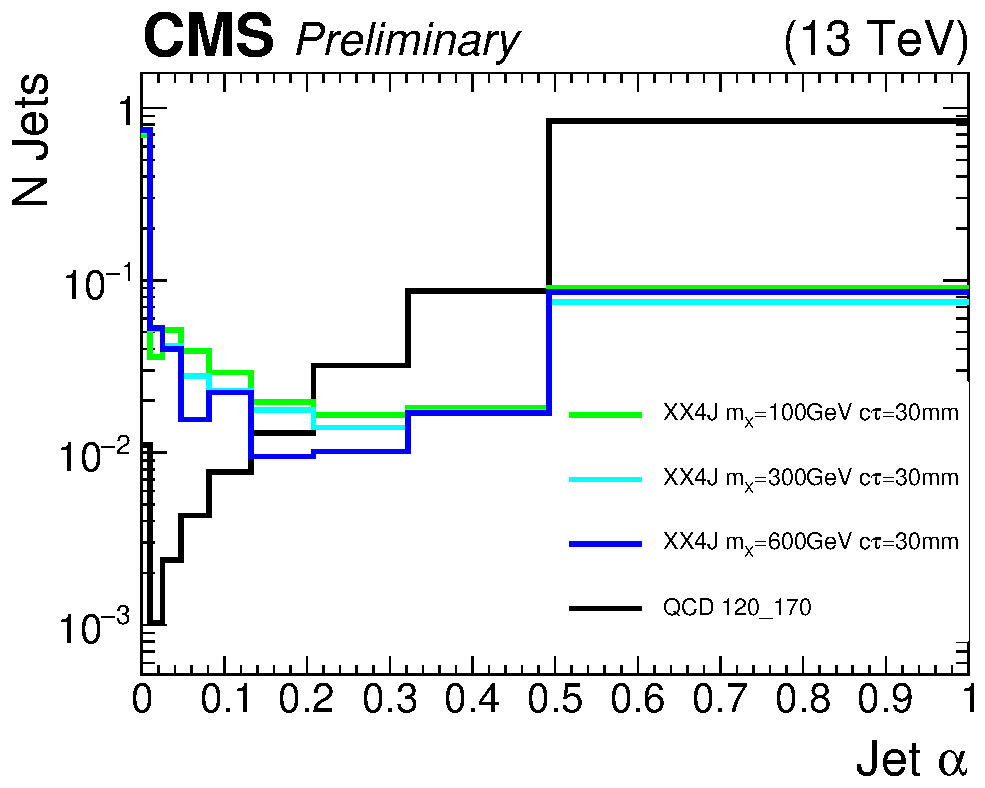
\includegraphics[width=.45\textwidth]{figures/an_jetid/VTX_MATCH_IP/XX4J_MASS_alpha}
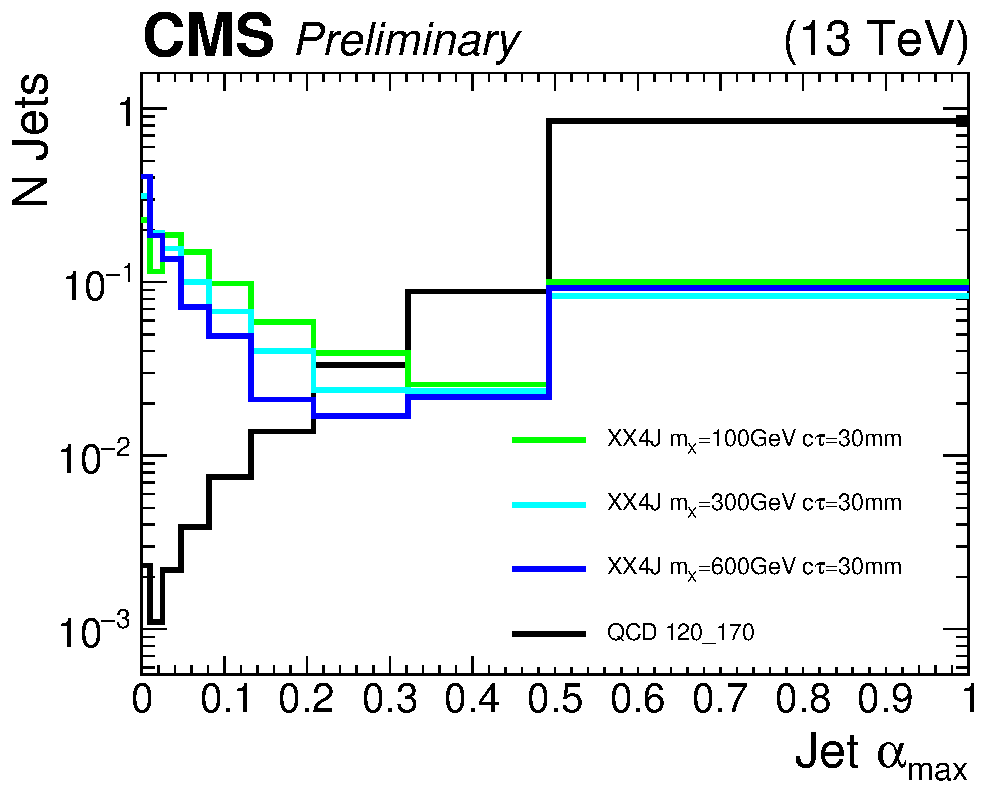
\includegraphics[width=.45\textwidth]{figures/an_jetid/VTX_MATCH_IP/XX4J_MASS_alphaMax}
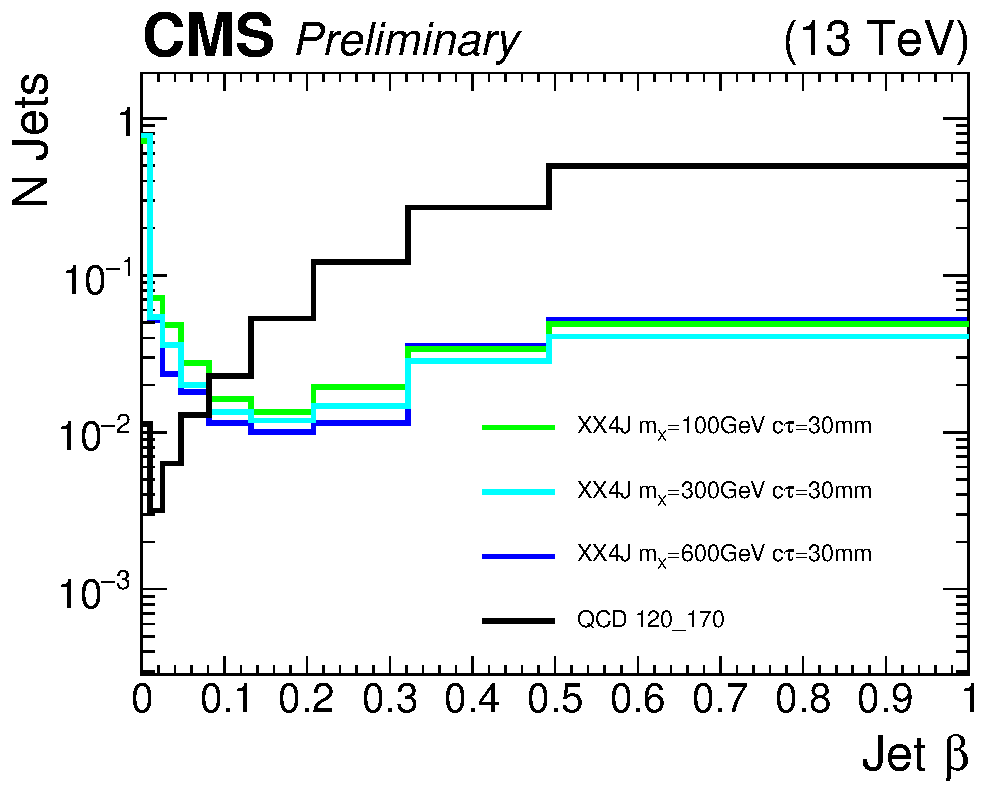
\includegraphics[width=.45\textwidth]{figures/an_jetid/VTX_MATCH_IP/XX4J_MASS_beta}
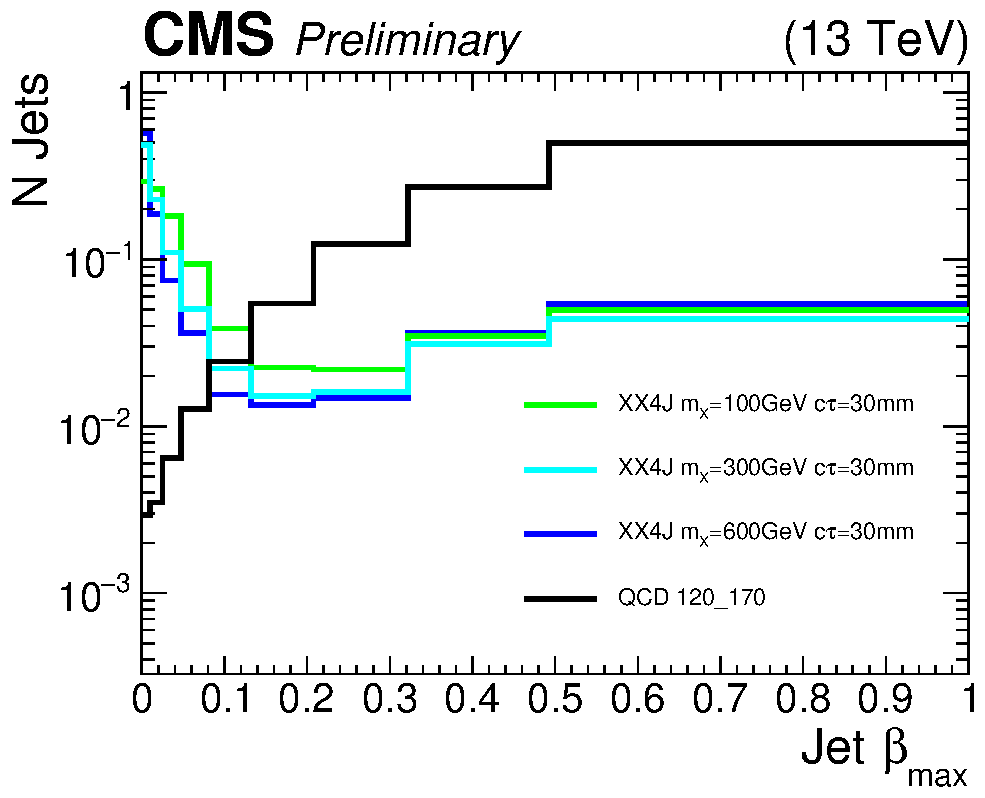
\includegraphics[width=.45\textwidth]{figures/an_jetid/VTX_MATCH_IP/XX4J_MASS_betaMax}
\end{center}
\caption{$\alpha, \alpha_{max}, \beta, \beta_{max}$ when varying the mass of the decaying $X^0$}
\label{fig:xx4j_mass_alpha_beta}
\end{figure}

Jets decaying displaced from the primary vertex are unlikely to contain tracks 
included in the event's primary vertex fit when a beam spot constraint is included.
QCD jets, expect the majority of their tracks to be from either the true primary vertex or a pile up vertex.
For a given jet $\alpha(PV)$ is calculated as the sum is taken over tracks matching in $\Delta R< 0.4$ between two
collections of tracks: the tracks in the specified primary vertex and tracks from the \texttt{generalTracks} collection. 
The sum is restricted to tracks with $p_{t} > 1.0$ GeV. 

\begin{equation}
\alpha_{jet}(PV) = \frac{\sum_{i\in PV,tracks} p_{t}^i}{ \sum_{j\in generalTracks} p_{t}^j }
\end{equation}

If a single PV is selected for all jets in the event, PU jets which are not from this vertex can have signal-like $\alpha \approx 0$. 
To avoid this we define $\alpha_{max}$ for each jet individually selecting the primary vertex with
the largest contribution to the sum. The assumption is PU jets will have high $\alpha$ for at least one 
of the vertices. Many events with $\alpha = 0$ have $\alpha_{max} != 0$ as they originate
from a sub-leading vertex in the \texttt{offlinePrimaryVerticesWithBS} collection. 
Because the \textbf{GUN} samples typically have no reconstructed primary vertices (except in the
prompt case), these plots are not shown. 

A second jet variable $\beta(PV)$ and $\beta_{max}$ are defined similarly:

\begin{equation}
\beta_{jet}(PV) = \frac{\sum_{i \in PV,tracks} p_{t}^i}{p_{t,jet}}
\end{equation}

A comparison of the four variables: $\alpha, \alpha_{max}, \beta, \beta_{max}$ is shown in Fig. \ref{fig:xx4j_alpha_beta} varying 
the lifetime of the sample and in Fig. \ref{fig:xx4j_mass_alpha_beta} varying the mass for fixed lifetime. 

\begin{figure}
\begin{center}
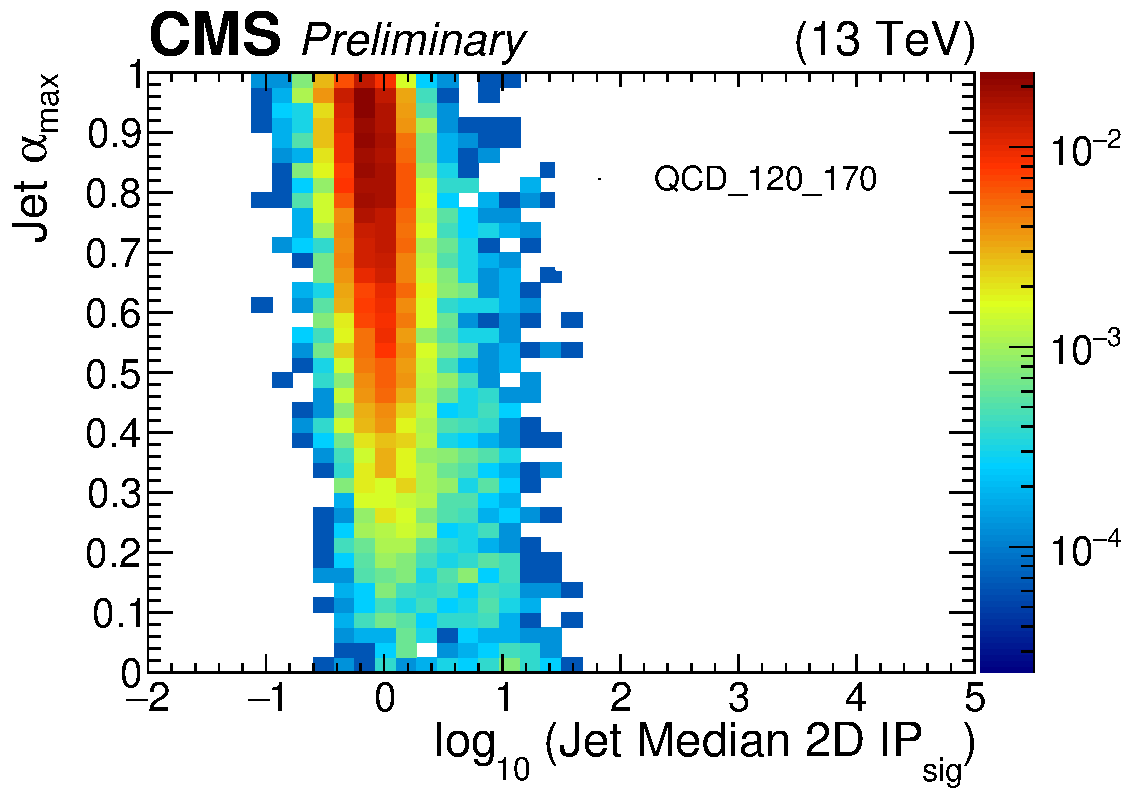
\includegraphics[width=.45\textwidth]{figures/an_jetid/VTX_MATCH_IP/QCD_2D_medianipsig_alpha}
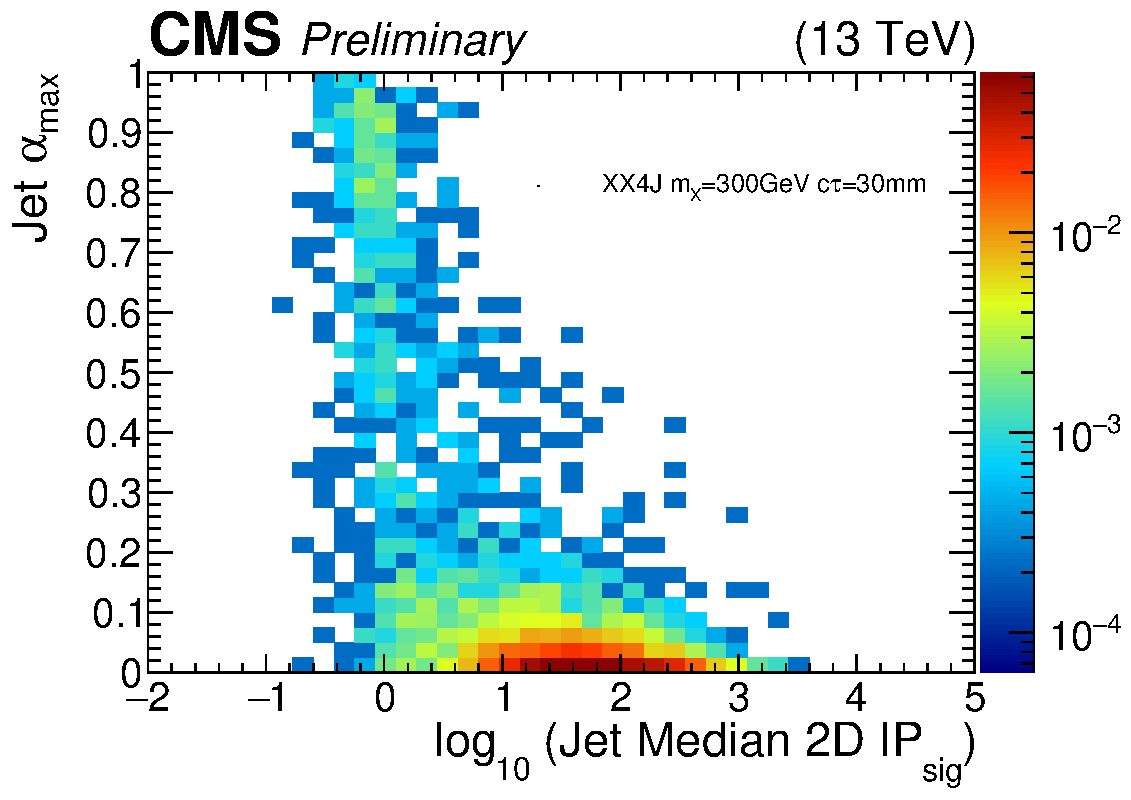
\includegraphics[width=.45\textwidth]{figures/an_jetid/VTX_MATCH_IP/XX4J_2D_medianipsig_alpha}
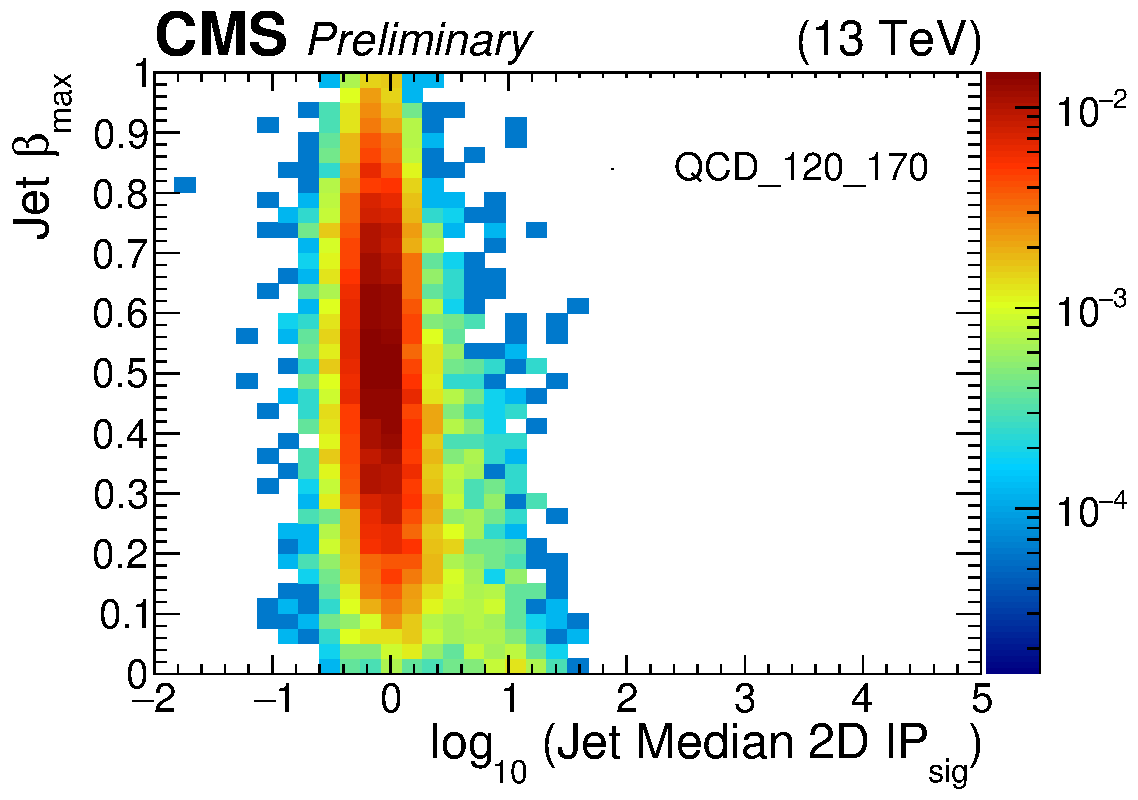
\includegraphics[width=.45\textwidth]{figures/an_jetid/VTX_MATCH_IP/QCD_2D_medianipsig_beta}
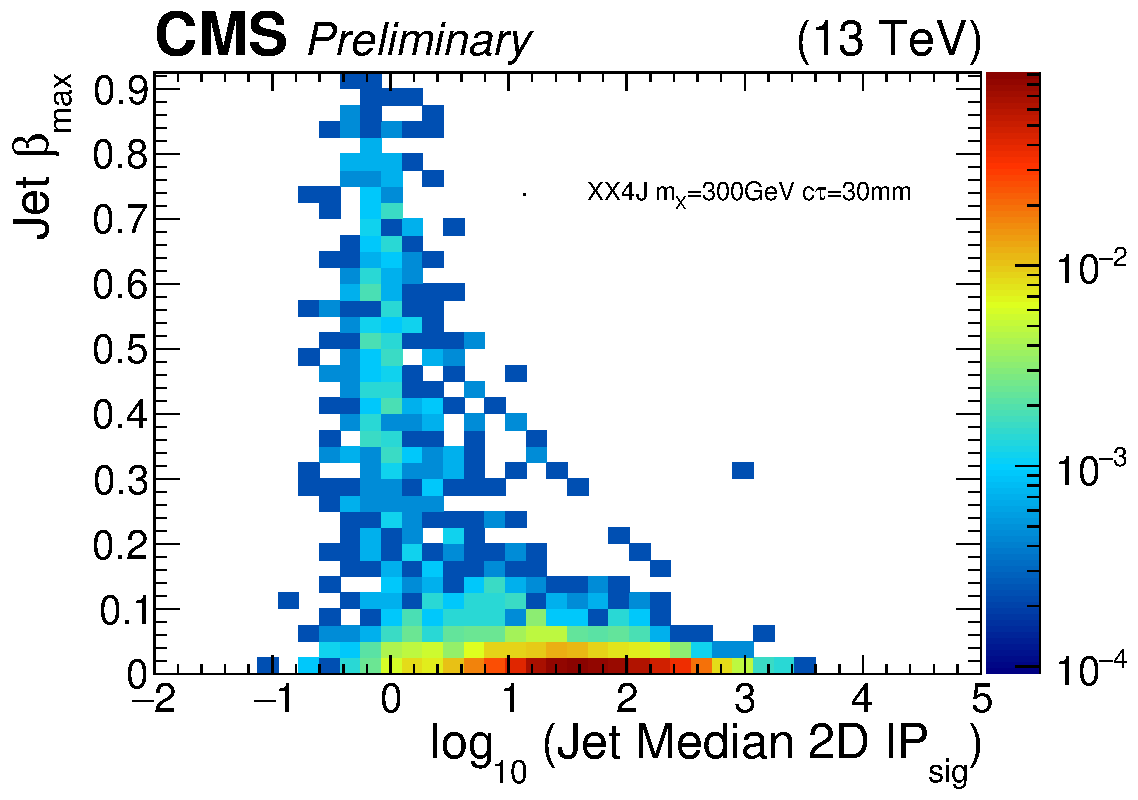
\includegraphics[width=.45\textwidth]{figures/an_jetid/VTX_MATCH_IP/XX4J_2D_medianipsig_beta}

\end{center}
\caption{(Left) The correlation between $\alpha_{max}$ and $\beta_{max}$ and median 2D IP significance for QCD (Right) The same for XX4J with $m_X=300$ GeV and $c\tau = 30$mm}
\label{fig:2d_alpha_beta_ipsig}
\end{figure}

Fig \ref{fig:2d_alpha_beta_ipsig} show $\alpha_{max}$ has small correlation in background with the median 2D IP significance
 and $\beta_{max}$ less so. This is because $\alpha_{max}$ is a function of the tracks matched to the jet, 
which are utilized in the median IP significance calculation. At low values of $\alpha_{max}$ we find the best separation
between between signal and background.


\subsection{Calo Jet Information}

\begin{figure}
\begin{center}
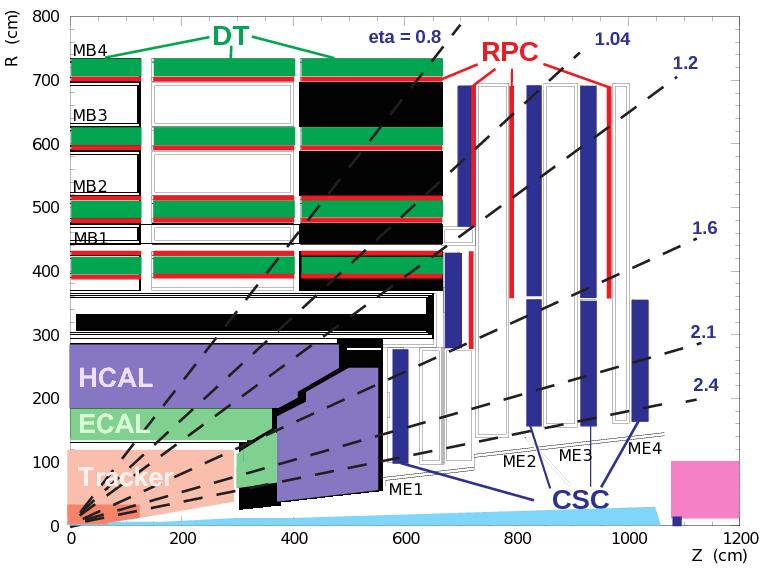
\includegraphics[width=.45\textwidth]{figures/an_jetid/DIAGRAMS/cms_slice}
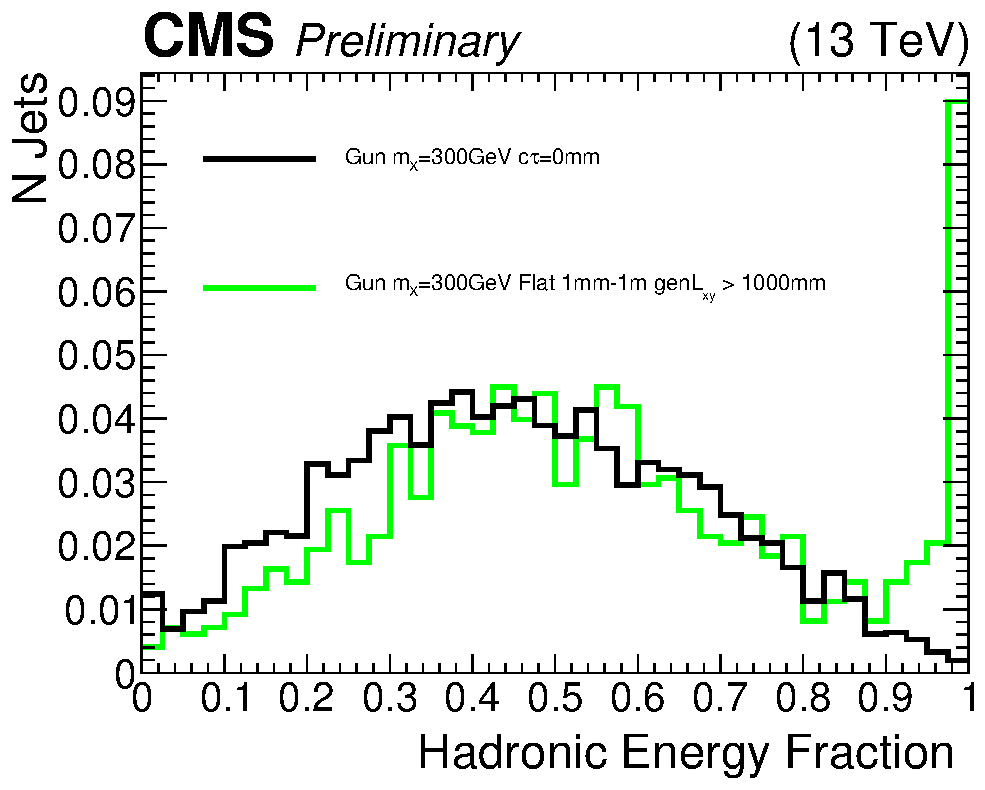
\includegraphics[width=.45\textwidth]{figures/an_jetid/VTX_MATCH_IP/GUN_hadronicFraction}
\end{center}
\caption{(Left) A longitudinal slice of the CMS detector showing the transverse coverage of the tracking layers. (Right) Hadronic fraction of jets in events with generator level requirement that the $X^{0}$ decay at a transverse distance
$L_{xy} > 100$cm}
\label{fig:hadronicFraction}
\end{figure}

In the case which there are no tracks to identify the decay as displaced, we can utilize the high hadronic energy fraction
of jets that occur from decays in the hadronic calorimeter. Fig. \ref{fig:hadronicFraction} applies a generator level
cut on the transverse decay distance of $L_{xy} > 100$ cm to insure that the decay occurs outside of the tracker.
